\documentclass[12pt]{report}
\usepackage[utf8]{inputenc}
\usepackage[T1]{fontenc}
\usepackage[french]{babel}
\usepackage{graphicx}
\usepackage{caption}
\usepackage{float}
\usepackage{geometry}
\usepackage{hyperref}
\usepackage{listings}
\geometry{a4paper, margin=2.5cm}

\begin{document}

\noindent
\begin{minipage}[c]{0.6\textwidth}
    \vspace{6mm}
    \raggedright
    Ministère de l'Enseignement Supérieur et de la Recherche Scientifique\\
    Institut International de Technologie à Sfax
\end{minipage}
\hfill
\begin{minipage}[c]{0.35\textwidth}
    \raggedleft
    
\includegraphics[width=0.9\textwidth]{LogoIIT}
\end{minipage}

\vspace{5mm}
\hrule
\vspace{2.5cm}

\begin{center}
    {\fontsize{25pt}{30pt}\selectfont \textbf{\textsc{Rapport du projet ERP}}}
    
    \vspace{2cm}
    
    {\fontsize{20pt}{24pt}\selectfont \textbf{Réalisation d’un processus de vente avec Odoo 18}}

    \vspace{4cm}

    {\fontsize{15pt}{18pt}\selectfont \textbf{Enseignant :}}\\[0.5em]
    {\fontsize{12pt}{16pt} \textbf{Dr. Mohamed MANAA}}

    \vspace{4cm}
    
    {\fontsize{15pt}{18pt}\selectfont Élaboré par :}\\[0.5em]
    {\fontsize{12pt}{16pt} Chedy Chaaben}
    
    \vspace{1cm}
    
    {\fontsize{16pt}{20pt}\selectfont Année universitaire : 2024/2025}
\end{center}

\newpage

\tableofcontents
\newpage


\chapter{Introduction}

Ce rapport décrit la mise en œuvre d’un processus de vente au sein de l’ERP Odoo, en s’appuyant sur le modèle de la société tunisienne Mytek, spécialisée dans la vente de matériel informatique.

L’objectif principal de ce projet est double :
\begin{itemize}
    \item Reproduire une interface utilisateur similaire à celle du site e-commerce de Mytek ;
    \item Intégrer une solution de paiement en ligne adaptée au marché tunisien, en l’occurrence le module Konnect payments.
\end{itemize}

Ce projet offre l’opportunité de mettre en pratique plusieurs modules d’Odoo dans un contexte concret de digitalisation des processus commerciaux.

\chapter{Description du processus}

\section{Odoo ERP}

Odoo est un logiciel ERP open source et modulaire, permettant une gestion intégrée de l’ensemble des activités d'une entreprise. Il propose un très grand nombre de modules qui couvrent une large variété de processus métiers tels que la gestion des ventes, des stocks, des finances, des ressources humaines, et bien d'autres.

Le grand avantage d’Odoo réside dans sa modularité : chaque entreprise peut choisir d’implémenter les modules qui lui sont les plus adaptés, tout en ayant la possibilité de les intégrer de manière transparente dans un écosystème commun. L’interface est intuitive et les données sont centralisées, ce qui améliore la fluidité du processus décisionnel et permet une gestion plus efficace.

\section{Pourquoi Mytek ?}

Mytek est un acteur majeur du e-commerce informatique en Tunisie, offrant une large gamme de produits technologiques allant des ordinateurs aux périphériques. Son site web présente une structure claire et une ergonomie fluide, rendant l’expérience d’achat en ligne agréable pour les utilisateurs. Le site met en avant des catégories de produits, des promotions, ainsi que des filtres de recherche performants.

Cloner ce site pour un projet d’intégration avec Odoo représente un excellent exercice de reproduction fonctionnelle et d’adaptation des modules ERP à un contexte spécifique. Cela permet de mettre en pratique la gestion des ventes, la gestion des stocks, ainsi que l’intégration de solutions de paiement en ligne adaptées au marché tunisien.

\section{Pourquoi Odoo ?}

Odoo est choisi pour ce projet en raison de sa flexibilité et de son écosystème intégré qui permet de connecter tous les aspects de la gestion de l’entreprise. Odoo propose une large gamme de modules qui rendent la gestion d'une entreprise aussi simple qu’un clic. Que ce soit pour la gestion des ventes, la gestion de la comptabilité ou l'automatisation du service client, Odoo permet de centraliser et d'automatiser de nombreuses tâches, réduisant ainsi la charge administrative.

Les modules d’Odoo permettent d'accompagner les entreprises dans leur mise en place, en leur permettant de se concentrer pleinement sur leur cœur de métier. Par exemple, le module de gestion des ventes permet non seulement de créer et suivre les commandes, mais aussi de gérer les stocks, de traiter les paiements et de gérer la relation client. Grâce à son écosystème intégré et flexible, Odoo facilite l’automatisation des tâches, améliore l’efficacité et favorise la croissance.

\chapter{Modélisation BPMN}

Le processus de vente dans Odoo a été modélisé à l’aide de la notation BPMN (Business Process Model and Notation), ce qui permet de visualiser les différentes étapes du processus de commande et de vente. Le diagramme BPMN ci-dessous montre les différentes étapes suivies par l’entreprise, de la commande initiale du client jusqu’à la confirmation du paiement et la préparation de l’expédition.

\begin{figure}[H]
    \centering
    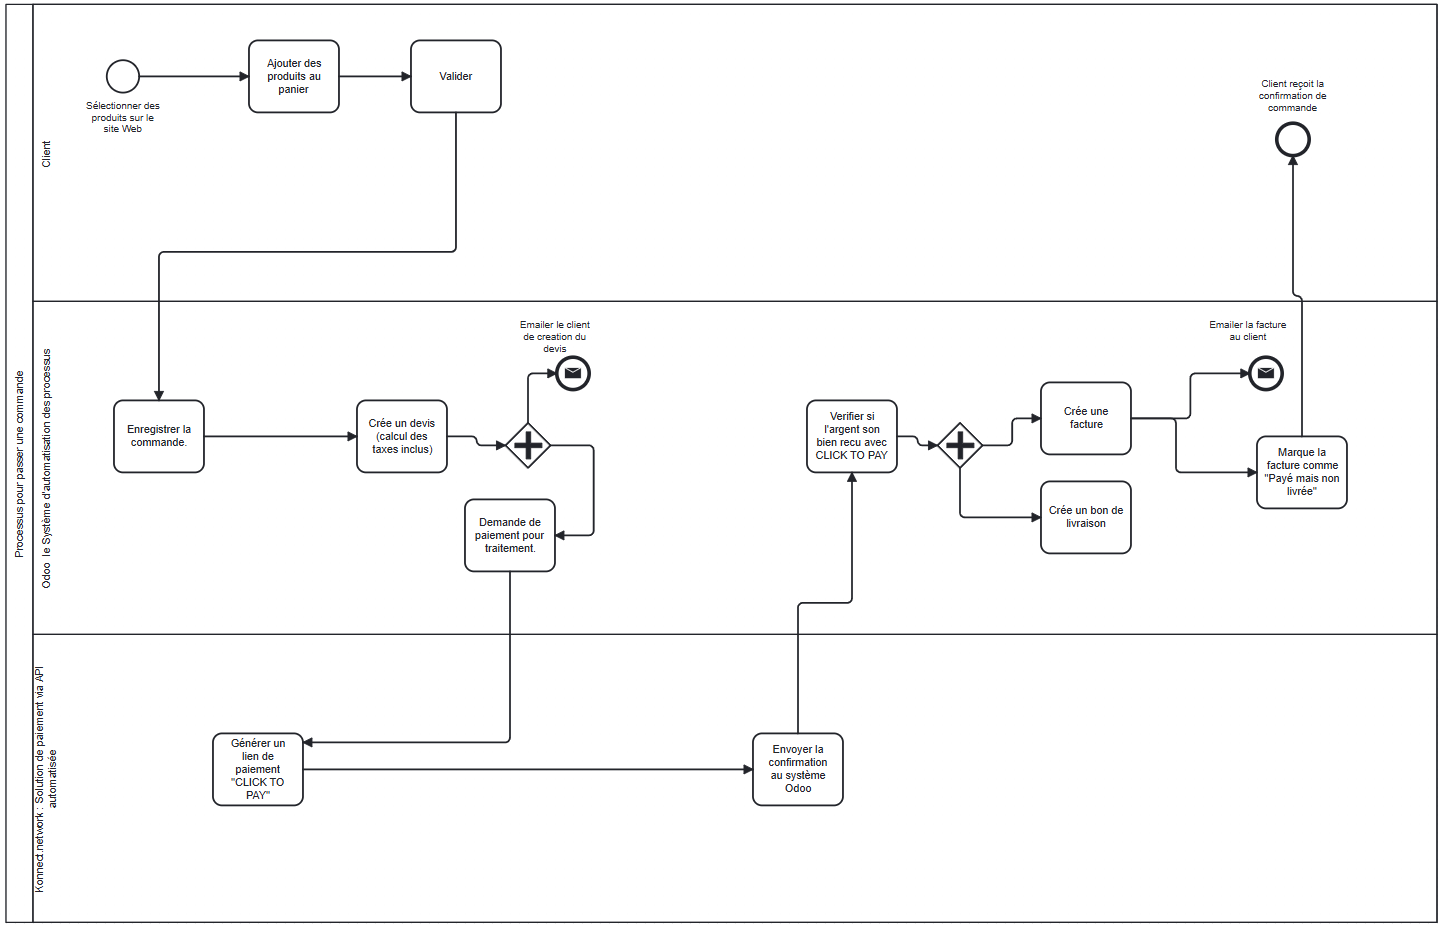
\includegraphics[width=0.6\textheight]{images/BPMN.PNG}
    \caption{Diagramme BPMN du processus PASSER UNE COMMANDE}
    \label{fig:bpmn}
\end{figure}

Le diagramme BPMN ci-dessus illustre les actions principales dans le processus de vente :

\begin{itemize}
    \item \textbf{Création d'un compte client} : Un nouveau client s'inscrit sur le site ou se connecte à son compte existant pour commencer la commande.
    \item \textbf{Sélection des produits} : Le client parcourt les catégories de produits disponibles et les ajoute à son panier.
    \item \textbf{Validation de la commande} : Après avoir vérifié les produits dans son panier, le client confirme sa commande.
    \item \textbf{Choix du mode de paiement} : Le client sélectionne une méthode de paiement (par exemple, carte bancaire, paiement Konnect).
    \item \textbf{Traitement de la commande} : Odoo génère un bon de commande et initie les processus nécessaires à la préparation de la commande (vérification du stock, gestion des expéditions, etc.).
    \item \textbf{Confirmation du paiement} : Une fois le paiement validé, le statut de la commande est mis à jour et l’expédition peut commencer.
    \item \textbf{Expédition et livraison} : Le produit est expédié et le client est informé de l'état d'avancement de sa commande.
    \item \textbf{Facturation} : Une facture est générée automatiquement dans le système Odoo pour clôturer la vente.
\end{itemize}

Ce modèle BPMN permet de comprendre les interactions entre les différents acteurs (client, système Odoo, personnel RH, etc.) et comment les tâches sont automatisées pour améliorer l'efficacité et la rapidité du processus de vente.

\chapter{Réalisation technique}

Ce chapitre détaille les étapes techniques de mise en place, de personnalisation et de configuration du projet réalisé avec Odoo, en passant par l'installation initiale jusqu’à l’intégration du paiement en ligne.

\section{Installation et configuration}

L'installation locale d'Odoo a été effectuée en utilisant la version \textbf{18.0 Community Edition}. L'environnement de développement comprend :

\begin{itemize}
\item \textbf{Système d’exploitation} : Windows 10 pro
\end{itemize}

Après l'installation, les modules nécessaires (site web, ventes, RH, inventaire, etc.) ont été activés pour permettre la personnalisation et l’ajout des fonctionnalités spécifiques au projet.

\section{Personnalisation du site web}

La page d’accueil du site a été modifiée afin de refléter l’image de l’entreprise et améliorer l’expérience utilisateur.

\begin{itemize}
\item Modification du titre principal et des images d’en-tête.
\item Personnalisation des boutons : textes, couleurs et liens.
\end{itemize}

\begin{figure}[H]
\centering
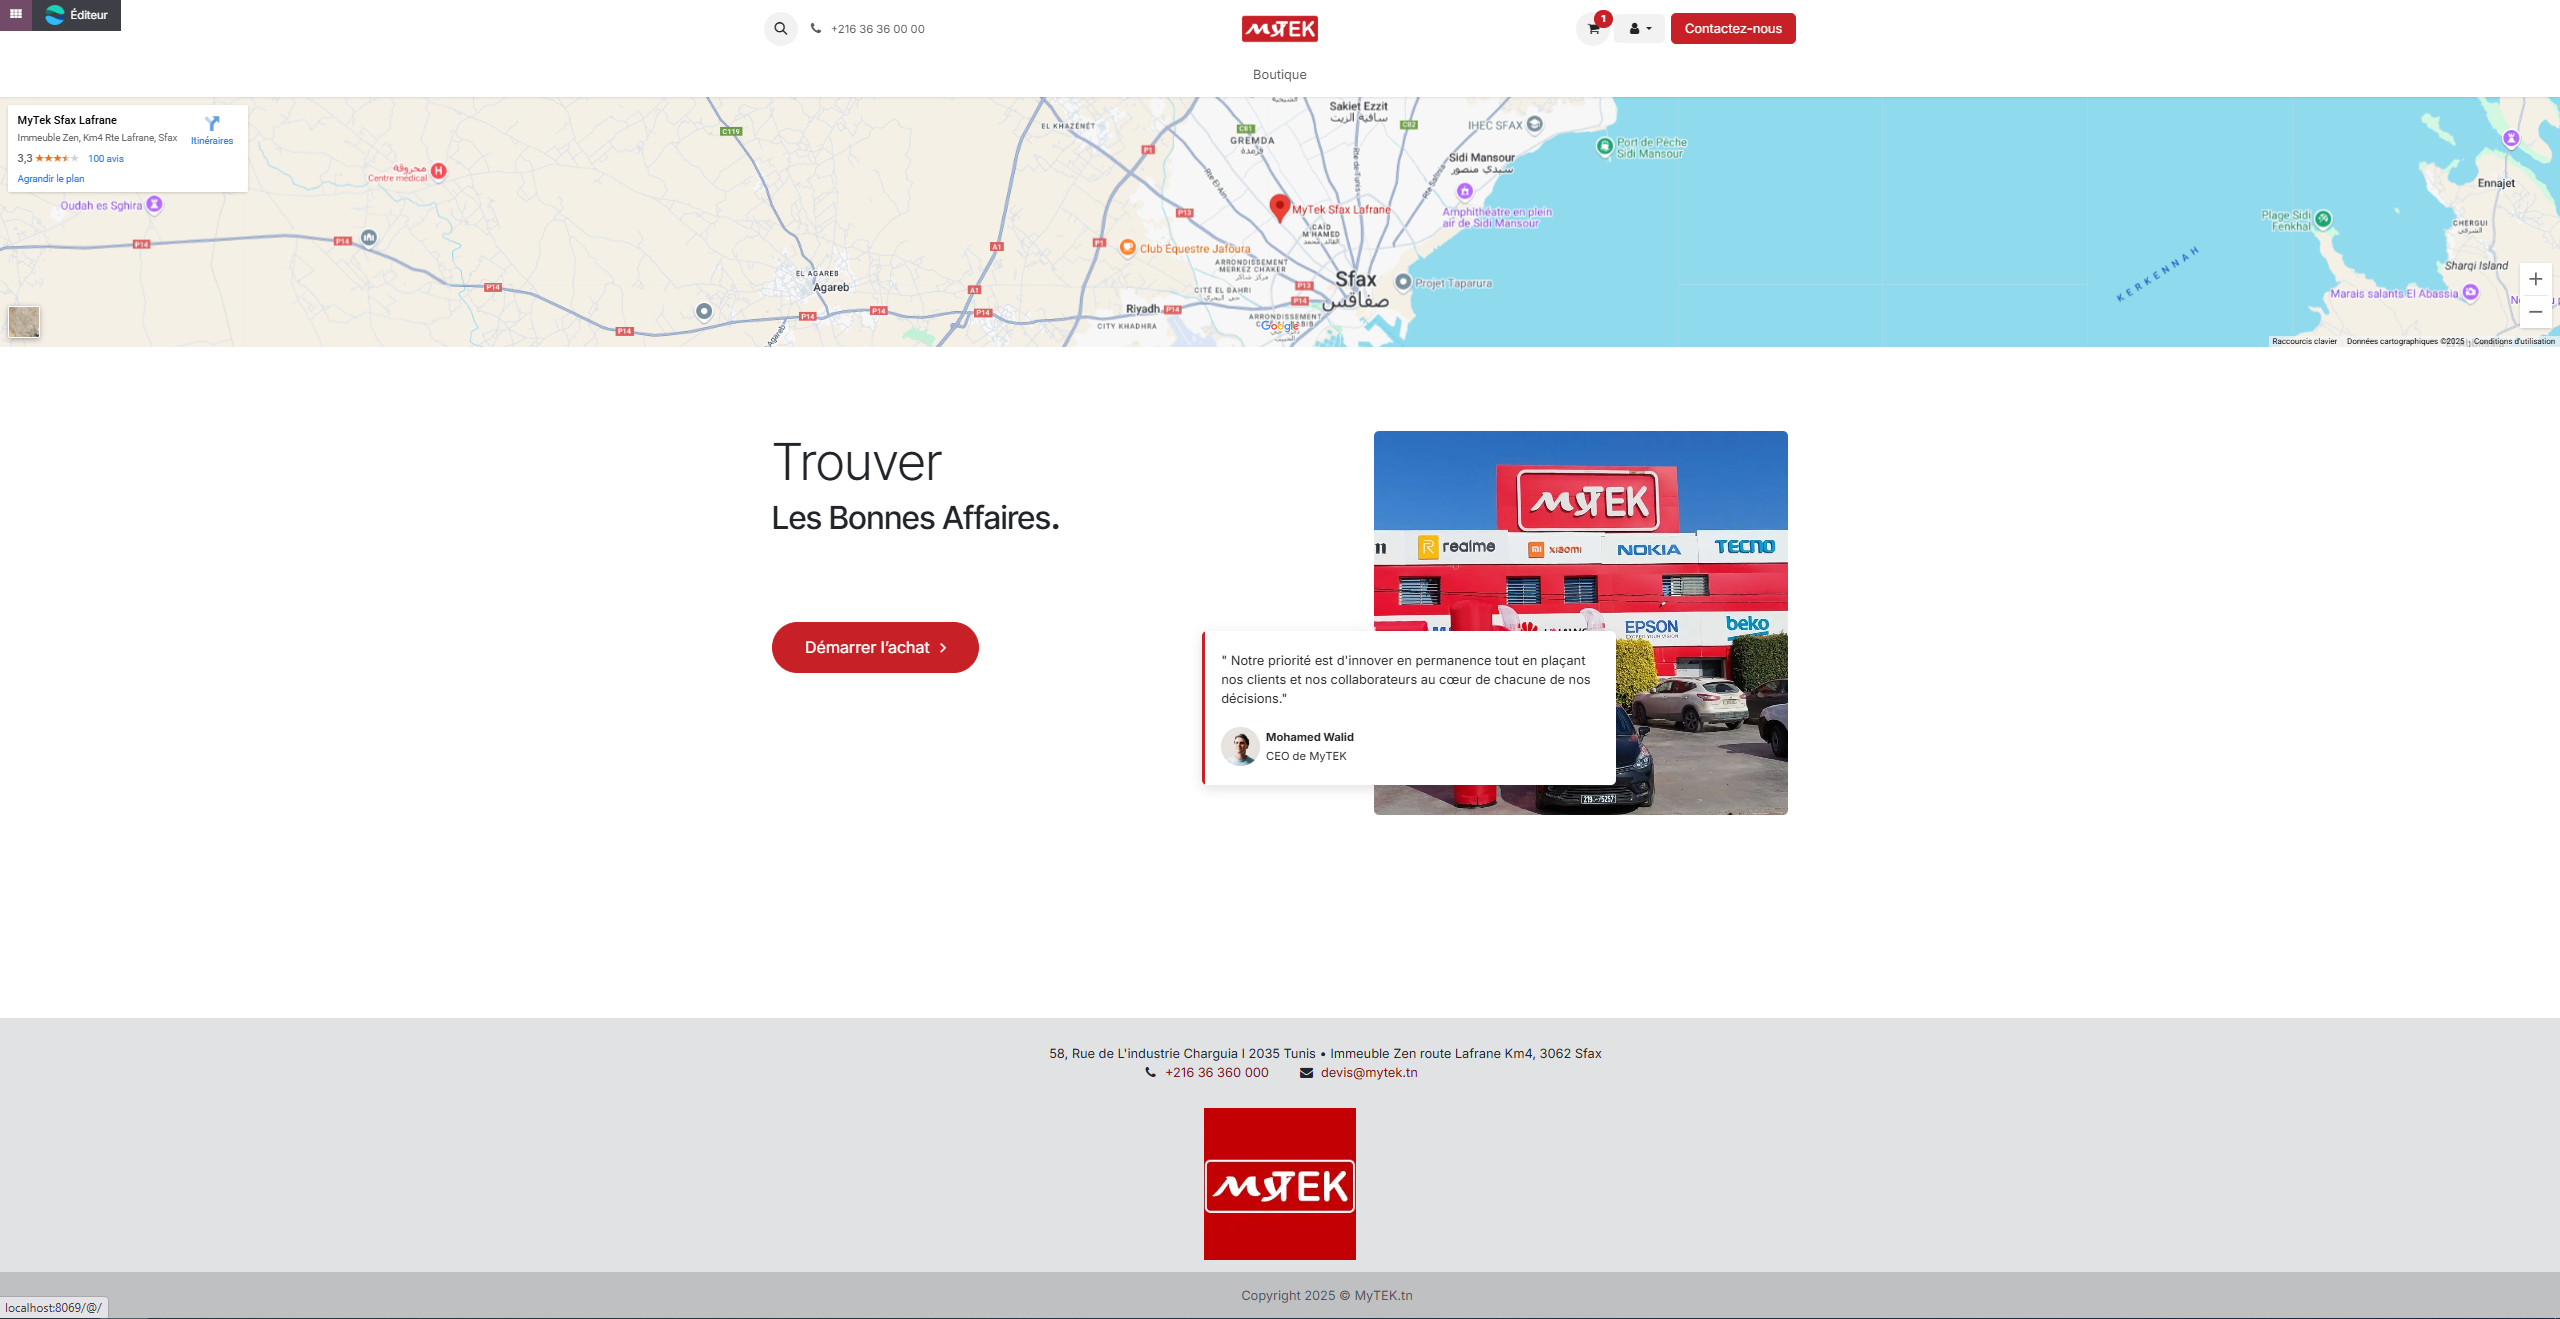
\includegraphics[width=0.8\textwidth]{images/interfaces/page_acceuil.PNG}
\caption{Page d'accueil après modification}
\end{figure}
\section{Ajout de produits}

Afin d'alimenter le site en produits, la méthode d'importation automatisée via un fichier Excel a été choisie. Cette approche permet de gagner du temps et de garantir une structuration uniforme des données. Le fichier Excel utilisé pour l'importation a été généré en suivant le squelette proposé par Odoo, qui définit la structure et les champs nécessaires à une bonne intégration des produits dans le système.

\subsection{Préparation du fichier Excel}

Le fichier Excel contient plusieurs colonnes essentielles, telles que :
\begin{itemize}
    \item \textbf{ID} : L'identifiant unique attribué à chaque produit. Cet ID est utilisé pour référencer le produit dans le système, afin de faciliter sa gestion.
    \item \textbf{Nom du produit} : Le nom exact du produit tel qu'il apparaîtra sur le site, utilisé pour identifier le produit dans les recherches et sur les pages de détails.
    \item \textbf{Type} : La catégorie ou le type de produit, comme "Ordinateur", "Accessoire", "Périphérique", etc. Cela permet de mieux organiser les produits dans les différentes sections du site.
    \item \textbf{Référence} : Le numéro de référence ou SKU (Stock Keeping Unit) unique, permettant d'identifier précisément chaque produit et de le gérer efficacement dans le stock.
    \item \textbf{Barcode} : Le code-barres associé au produit, qui peut être scanné pour faciliter le suivi en magasin ou lors des processus de gestion des stocks.
    \item \textbf{Prix de vente} : Le prix auquel le produit sera vendu aux clients sur le site. Ce prix peut inclure des taxes et des frais supplémentaires selon les paramètres de l'entreprise.
    \item \textbf{Coût} : Le coût d'acquisition ou de fabrication du produit, utilisé pour calculer la marge bénéficiaire et optimiser la gestion des stocks.
    \item \textbf{Description} : Une description détaillée du produit, expliquant ses caractéristiques, ses avantages et toute autre information utile pour le consommateur. Cette description aide à améliorer l'expérience client et à faciliter la décision d'achat.
\end{itemize}


Ce fichier Excel est ensuite importé dans Odoo via le module de gestion des produits.

\begin{figure}[H]
\centering
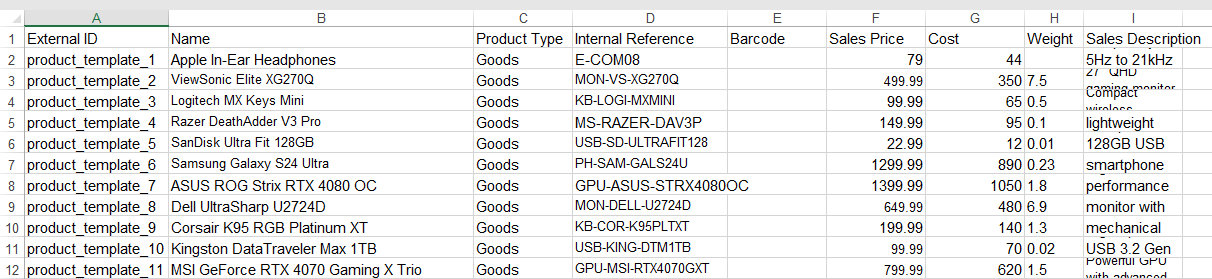
\includegraphics[width=0.8\textwidth]{images/ExcelODOO.PNG}
\caption{Fichier Excel importé dans Odoo}
\end{figure}

\subsection{Processus d'importation}

L'importation des produits dans Odoo est réalisée en utilisant la fonctionnalité d'importation de données du système. Une fois le fichier Excel prêt et vérifié, il suffit de suivre les étapes suivantes :
\begin{itemize}
    \item Accéder au module \texttt{Produits} dans Odoo.
    \item Sélectionner l'option d'importation depuis un fichier.
    \item Télécharger le fichier Excel préalablement préparé.
    \item Mapper les colonnes du fichier Excel avec les champs correspondants dans Odoo (par exemple, la colonne "Nom du produit" avec le champ "Nom" dans Odoo).
    \item Lancer l'importation et vérifier que les produits sont correctement ajoutés au système.
\end{itemize}

Cette méthode permet une insertion rapide et structurée d’un grand nombre d’articles, tout en minimisant le risque d'erreurs humaines qui pourrait survenir lors de la saisie manuelle.

\subsection{Avantages de l'importation via Excel}

L'utilisation de l'importation via Excel présente plusieurs avantages :
\begin{itemize}
    \item \textbf{Gain de temps} : Importer des centaines ou des milliers de produits en une seule fois est beaucoup plus rapide que de les ajouter un par un.
    \item \textbf{Automatisation} : Une fois le fichier préparé, l'importation est automatisée et ne nécessite qu'un minimum d'interventions manuelles.
    \item \textbf{Structuration uniforme} : Le fichier Excel suit un format standardisé, ce qui garantit que toutes les données sont uniformes et correctement formatées pour Odoo.
    \item \textbf{Facilité de mise à jour} : Si des modifications sont nécessaires (par exemple, ajustement des prix ou des quantités), elles peuvent être effectuées directement dans le fichier Excel et réimportées sans nécessiter de modifications manuelles dans l'interface d'Odoo.
\end{itemize}

En utilisant cette méthode, l'intégration des produits dans Odoo devient un processus rapide, précis et efficace.


\section{Gestion des employés}

Le module Ressources Humaines (RH) d’Odoo a été utilisé pour gérer les employés de l'entreprise. Ce module permet de centraliser toutes les informations relatives aux employés, comme leurs coordonnées, leurs contrats de travail, leurs absences et leurs performances. L'utilisation de ce module facilite également l'intégration des différents processus RH au sein de l'entreprise, en les automatisant et en offrant une vue d'ensemble en temps réel.

Afin de tester le système avec des données réalistes tout en respectant la confidentialité des employés, des informations et images de personnes fictives ont été générées à l’aide de l’intelligence artificielle. Ces données ont permis de simuler des scénarios réels sans compromettre la confidentialité ou la sécurité des informations personnelles.

Voici un exemple d’image générée par IA, représentant un employé fictif, utilisé dans le système pour tester la gestion des employés :

\begin{figure}[H]
\centering

\includegraphics[width=0.3\textwidth]{images/chatGPTEmployee.png}
\caption{Exemple d’image générée par IA pour un employé fictif}
\end{figure}

Ce processus permet d'assurer une gestion fluide et conforme tout en préservant la confidentialité des informations sensibles.



\section{Configuration du serveur SMTP Gmail}

Lors de la mise en place de l'ERP Odoo, un problème a été rencontré lors de l’envoi des e-mails depuis le système. Ce problème était lié à la configuration par défaut des serveurs de messagerie dans Odoo, ce qui a nécessité une configuration manuelle pour résoudre l'incident.

\begin{figure}[H]
\centering
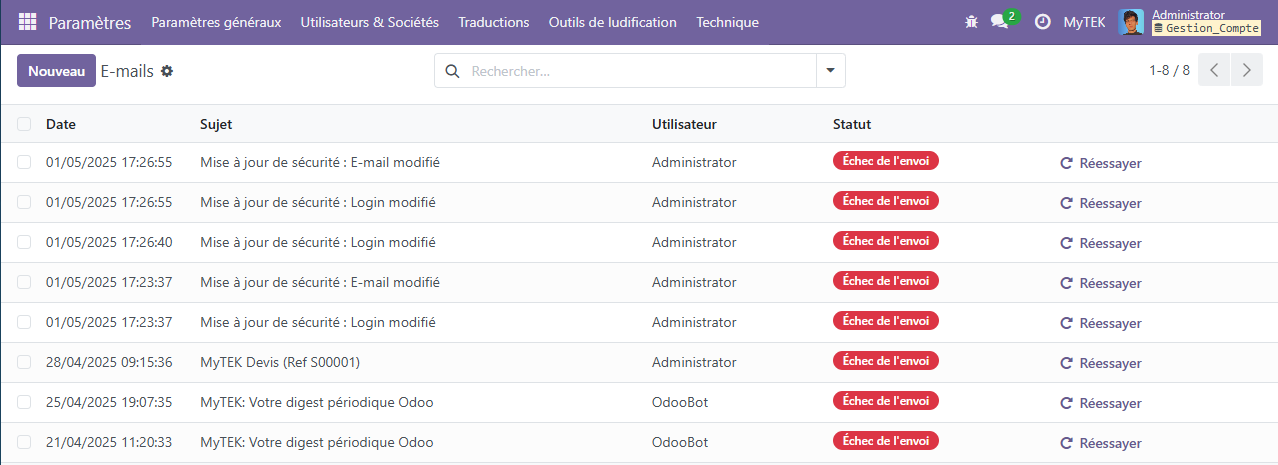
\includegraphics[width=0.8\textwidth]{images/email_ne_fonctionne_pas.PNG}
\caption{Erreur initiale d'envoi d'e-mails}
\end{figure}

\subsection{Solution apportée : utilisation du serveur SMTP de Gmail}

Pour contourner ce problème, l’envoi des courriels a été configuré via un serveur SMTP externe, en l’occurrence un compte Gmail personnel. Cette configuration a permis de garantir l'envoi des messages de manière fiable.

Les étapes pour configurer le serveur SMTP sont les suivantes :

\begin{itemize}
    \item \textbf{Serveur SMTP} : \texttt{smtp.gmail.com}
    \item \textbf{Port} : 587 (port utilisé pour les connexions sécurisées avec TLS)
    \item \textbf{Authentification} : L'adresse Gmail du compte et un mot de passe d’application spécifique (créé dans les paramètres de sécurité de Google).
\end{itemize}

La configuration de ces paramètres dans Odoo a permis de résoudre les problèmes d’envoi d’e-mails, notamment pour les notifications de commande et autres messages automatisés.

\begin{figure}[H]
\centering
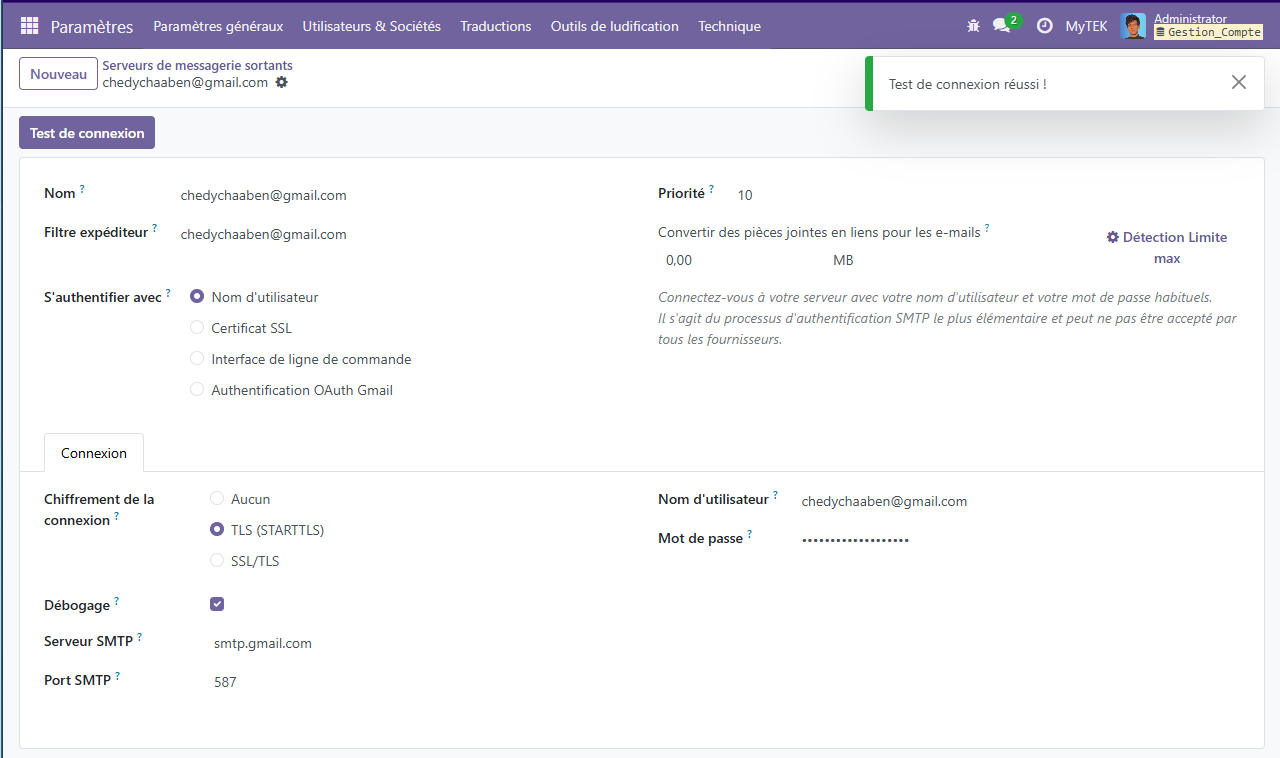
\includegraphics[width=0.8\textwidth]{images/configurationSMTPODOO.PNG}
\caption{Configuration SMTP dans Odoo}
\end{figure}

\subsection{Création du mot de passe d’application}

Google impose des règles de sécurité strictes pour l’accès aux comptes via des applications tierces. Afin de permettre à Odoo d’envoyer des e-mails, il a été nécessaire de créer un mot de passe spécifique pour l’application Gmail. Ce mot de passe d’application est un identifiant unique permettant à Odoo d’accéder au compte Gmail sans nécessiter de mot de passe principal.

Voici les étapes pour créer ce mot de passe dans le compte Google :

\begin{itemize}
    \item Aller dans les paramètres de sécurité de Google.
    \item Activer la vérification en deux étapes si elle n'est pas déjà activée.
    \item Créer un mot de passe d’application pour l'application "Autre (Nom personnalisé)".
\end{itemize}

Une fois le mot de passe généré, il a été intégré dans la configuration SMTP d'Odoo.

\begin{figure}[H]
\centering
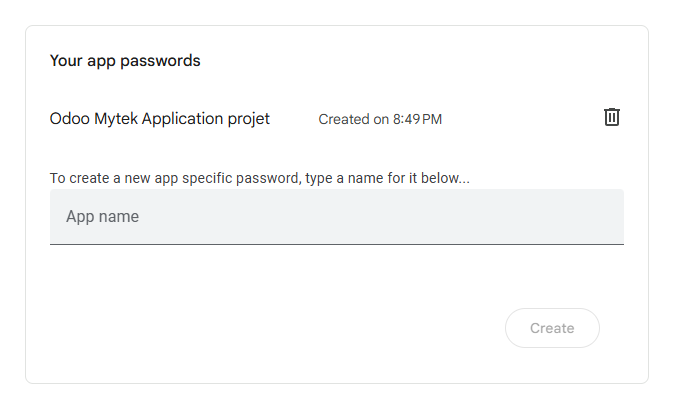
\includegraphics[width=0.8\textwidth]{images/google.PNG}
\caption{Création d’un mot de passe d’application dans Google}
\end{figure}

\subsection{Test de l'envoi d'e-mails}

Après avoir configuré le serveur SMTP et intégré le mot de passe d’application dans Odoo, un test d'envoi d'e-mail a été effectué pour vérifier que la configuration fonctionnait correctement.

Voici le résultat du test, montrant que l’envoi des e-mails a été réussi :

\begin{figure}[H]
\centering
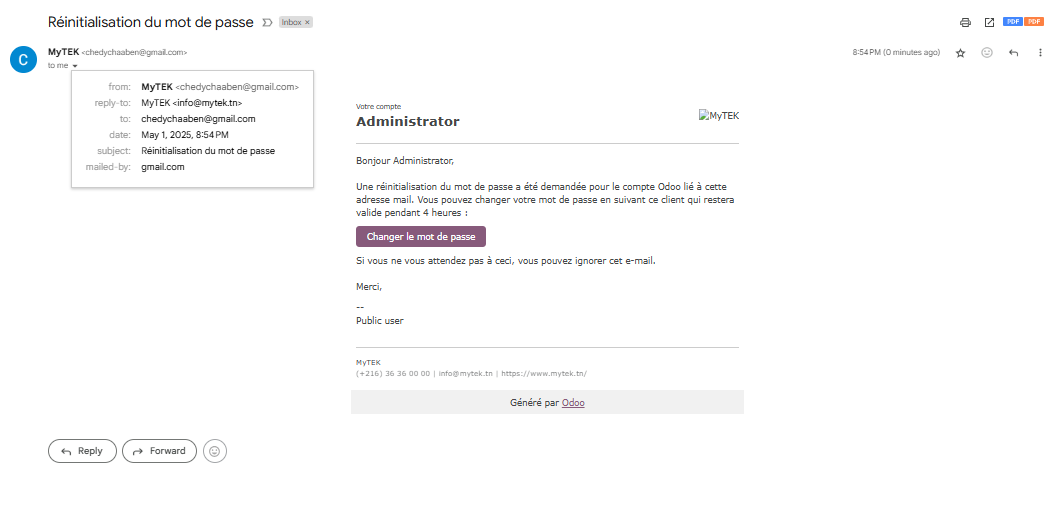
\includegraphics[width=0.8\textwidth]{images/MailOK.PNG}
\caption{Résultat après configuration du serveur de messagerie}
\end{figure}

Cette configuration permet désormais à Odoo d'envoyer automatiquement des notifications par e-mail, comme les confirmations de commande, les mises à jour d'expédition, et autres messages essentiels au bon fonctionnement du site de e-commerce.




\section{Intégration du paiement Konnect}

À l’origine, le site ne proposait aucun module de paiement, ce qui empêchait de finaliser les commandes en ligne. Une solution de paiement était donc indispensable pour permettre aux clients de régler leurs achats directement via le site. Après plusieurs recherches, une solution adaptée au marché tunisien a été trouvée : \textbf{le module Konnect}, proposé en tant qu'extension pour Odoo.

\subsection{Recherche de la solution de paiement}

Étant donné que le marché tunisien présente des spécificités en matière de solutions de paiement en ligne, il était nécessaire de sélectionner une option locale qui offre une intégration fluide avec l'ERP Odoo. Le module Konnect a été retenu en raison de sa compatibilité avec Odoo et de son intégration facile avec les systèmes de paiement locaux.

\begin{figure}[H]
\centering
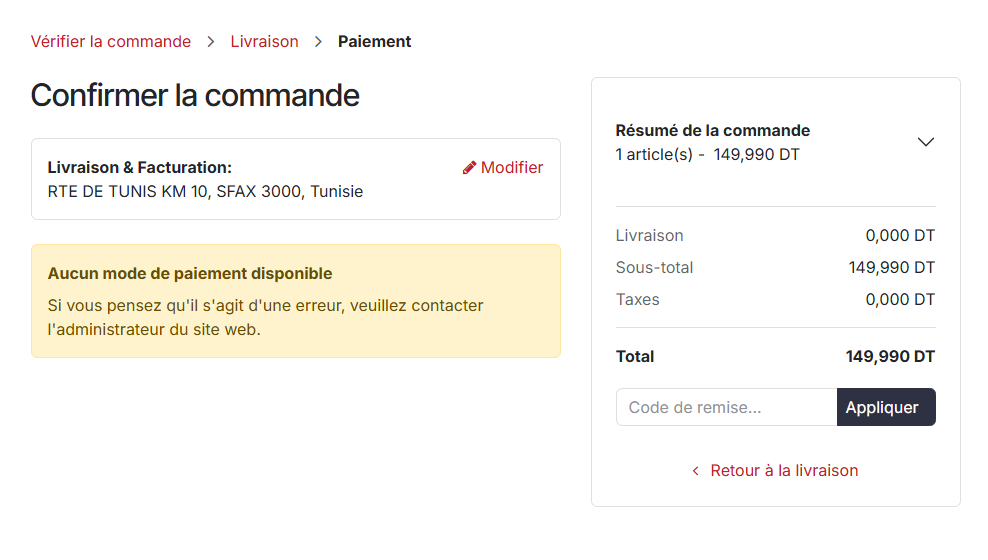
\includegraphics[width=0.8\textwidth]{images/site_sans_module_payement.PNG}
\caption{Site sans module de paiement}
\end{figure}

\subsection{Procédure d'intégration du module}

Une fois la solution Konnect choisie, il a fallu suivre plusieurs étapes pour l’intégrer dans le site :

\begin{itemize}
    \item \textbf{Création d'un compte Konnect} : Un compte professionnel a été créé sur la plateforme Konnect afin d'obtenir une clé API, nécessaire à l'activation du module.
    \item \textbf{Installation du module} : Le module Konnect a été installé dans Odoo via l'interface d'administration de l'ERP, en suivant la procédure fournie par le fournisseur du module.
    \item \textbf{Configuration de l'API} : La clé API générée sur le site Konnect a été intégrée dans Odoo pour lier les deux systèmes. Cela permet de traiter les paiements en toute sécurité.
\end{itemize}

Voici une capture d'écran du module Konnect, une fois activé dans Odoo :

\begin{figure}[H]
\centering
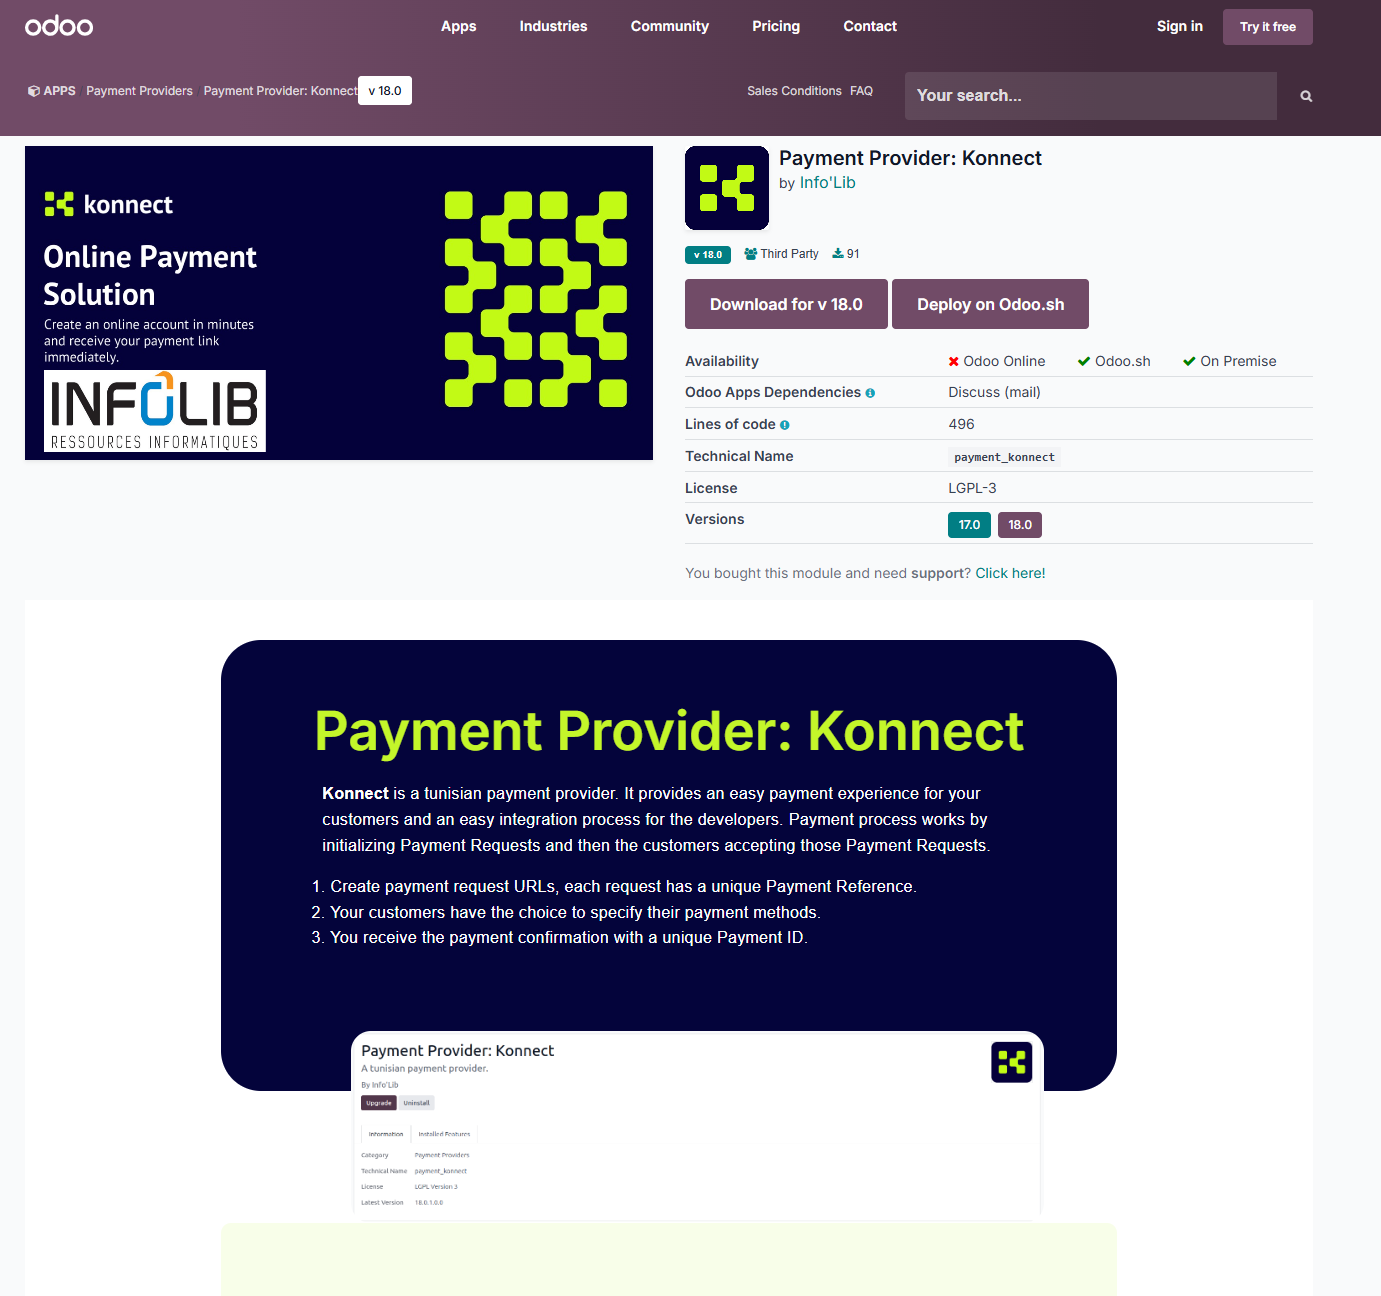
\includegraphics[width=1\textwidth]{images/Konnect Networks odoo module .PNG}
\caption{Module Konnect pour Odoo}
\end{figure}

\subsection{Obtention de la clé API}

Pour pouvoir effectuer des transactions sécurisées, il est essentiel d’obtenir une clé API depuis le site Konnect. Cette clé permet à Odoo de communiquer avec les serveurs Konnect pour autoriser les paiements.

\begin{figure}[H]
\centering
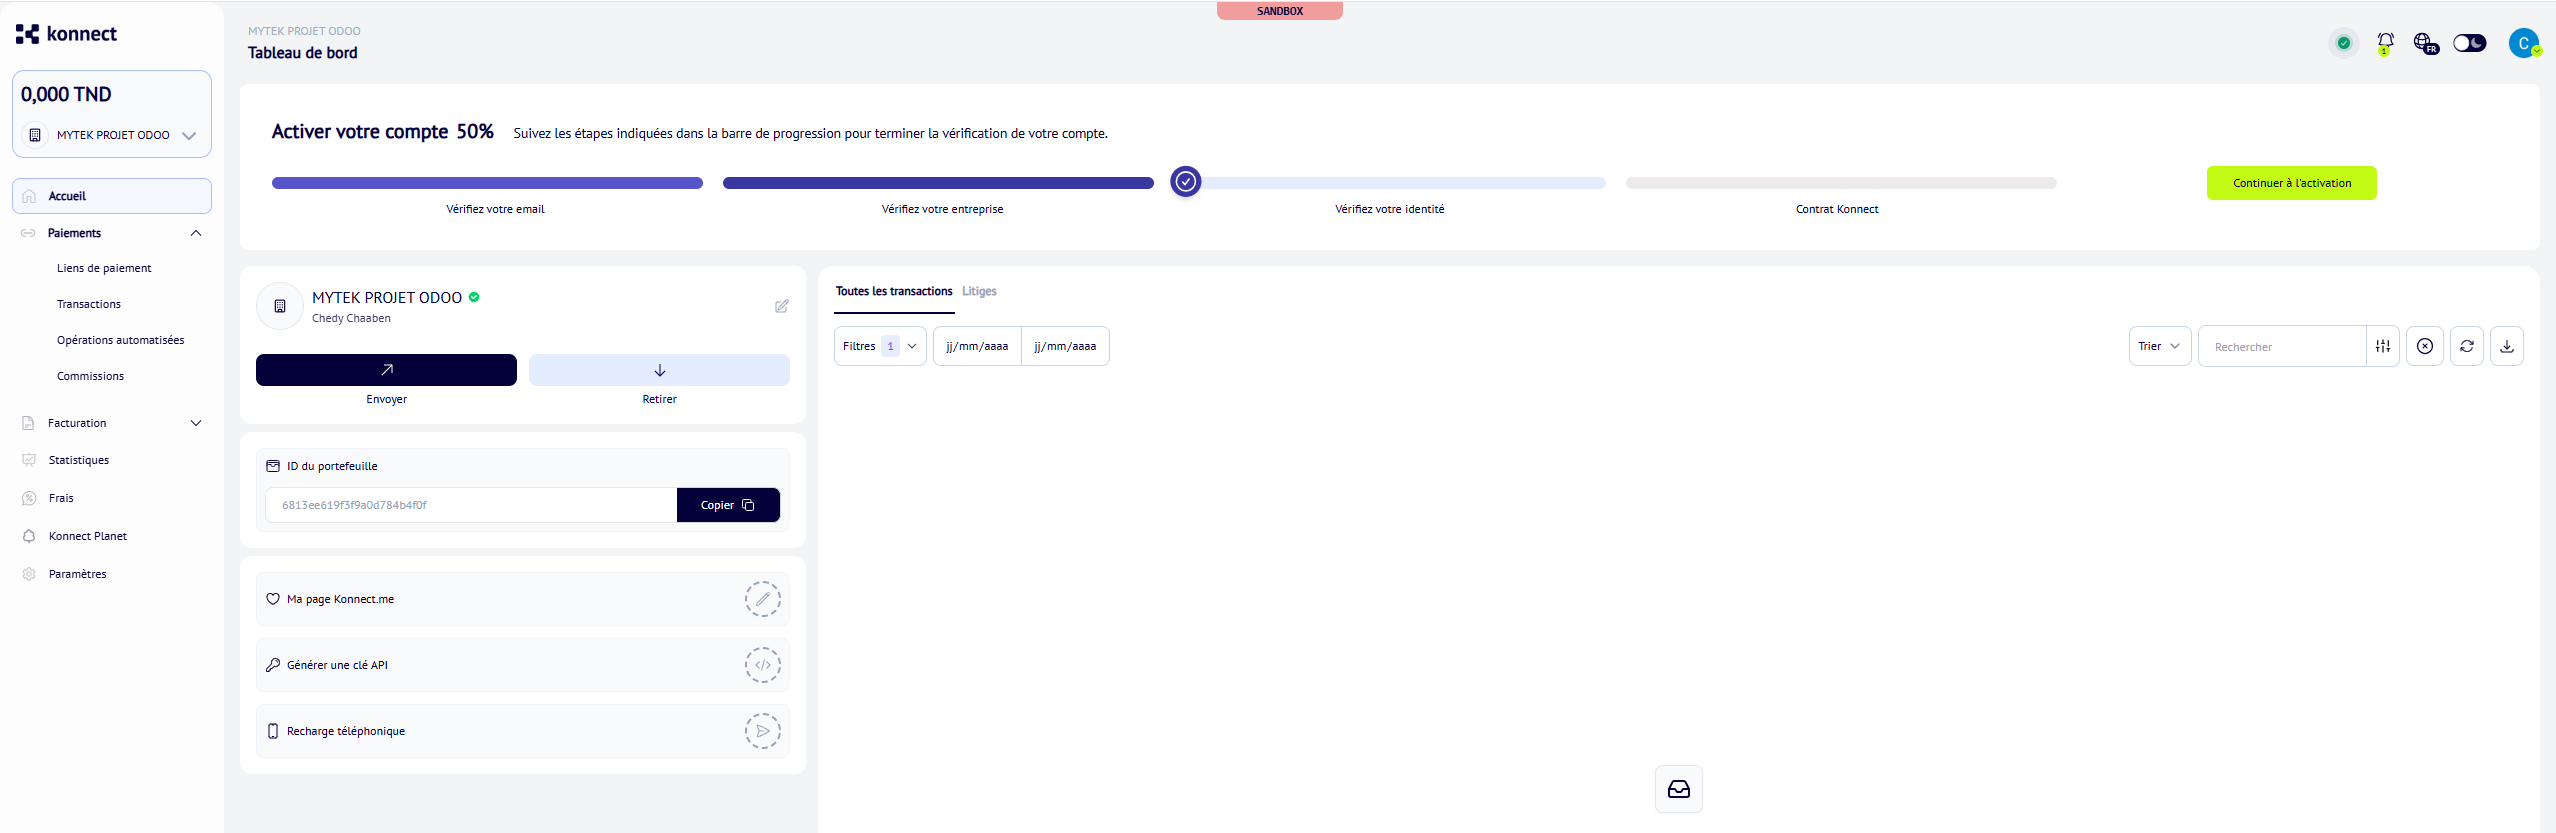
\includegraphics[width=1\textwidth]{images/api_key.PNG}
\caption{Obtention de la clé API Konnect}
\end{figure}

\subsection{Activation du module dans Odoo}

Une fois la clé API obtenue, le module Konnect a été activé dans Odoo en insérant cette clé dans les paramètres de configuration. L'activation a permis d'intégrer le paiement en ligne sur le site, permettant ainsi aux utilisateurs de procéder à des paiements directement lors de la commande.

\begin{figure}[H]
\centering
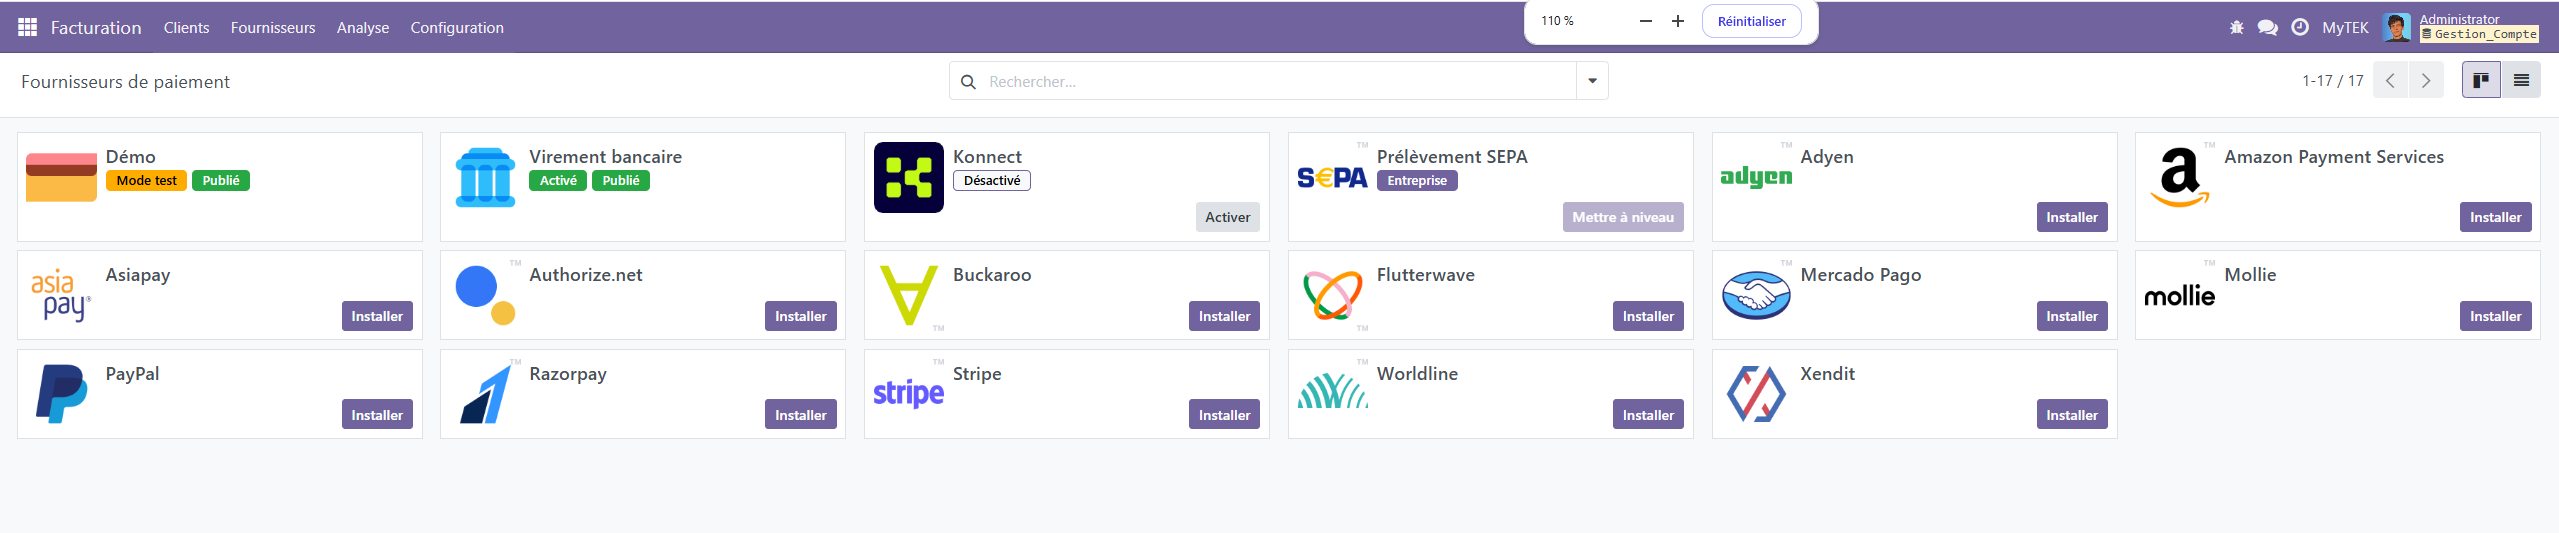
\includegraphics[width=1\textwidth]{images/activer payment.PNG}
\caption{Activation du module de paiement Konnect dans Odoo}
\end{figure}

Cette intégration permet désormais de gérer les paiements en ligne directement sur le site, ce qui améliore considérablement l’expérience utilisateur et complète le processus d’achat.



\chapter{Présentation du produit final}
Dans cette section, nous présentons le produit final à l’aide de plusieurs captures d’écran du site web développé. Ces images illustrent les principales fonctionnalités, l’interface utilisateur, ainsi que l’expérience de navigation offerte.

\begin{figure}[H]
    \centering
    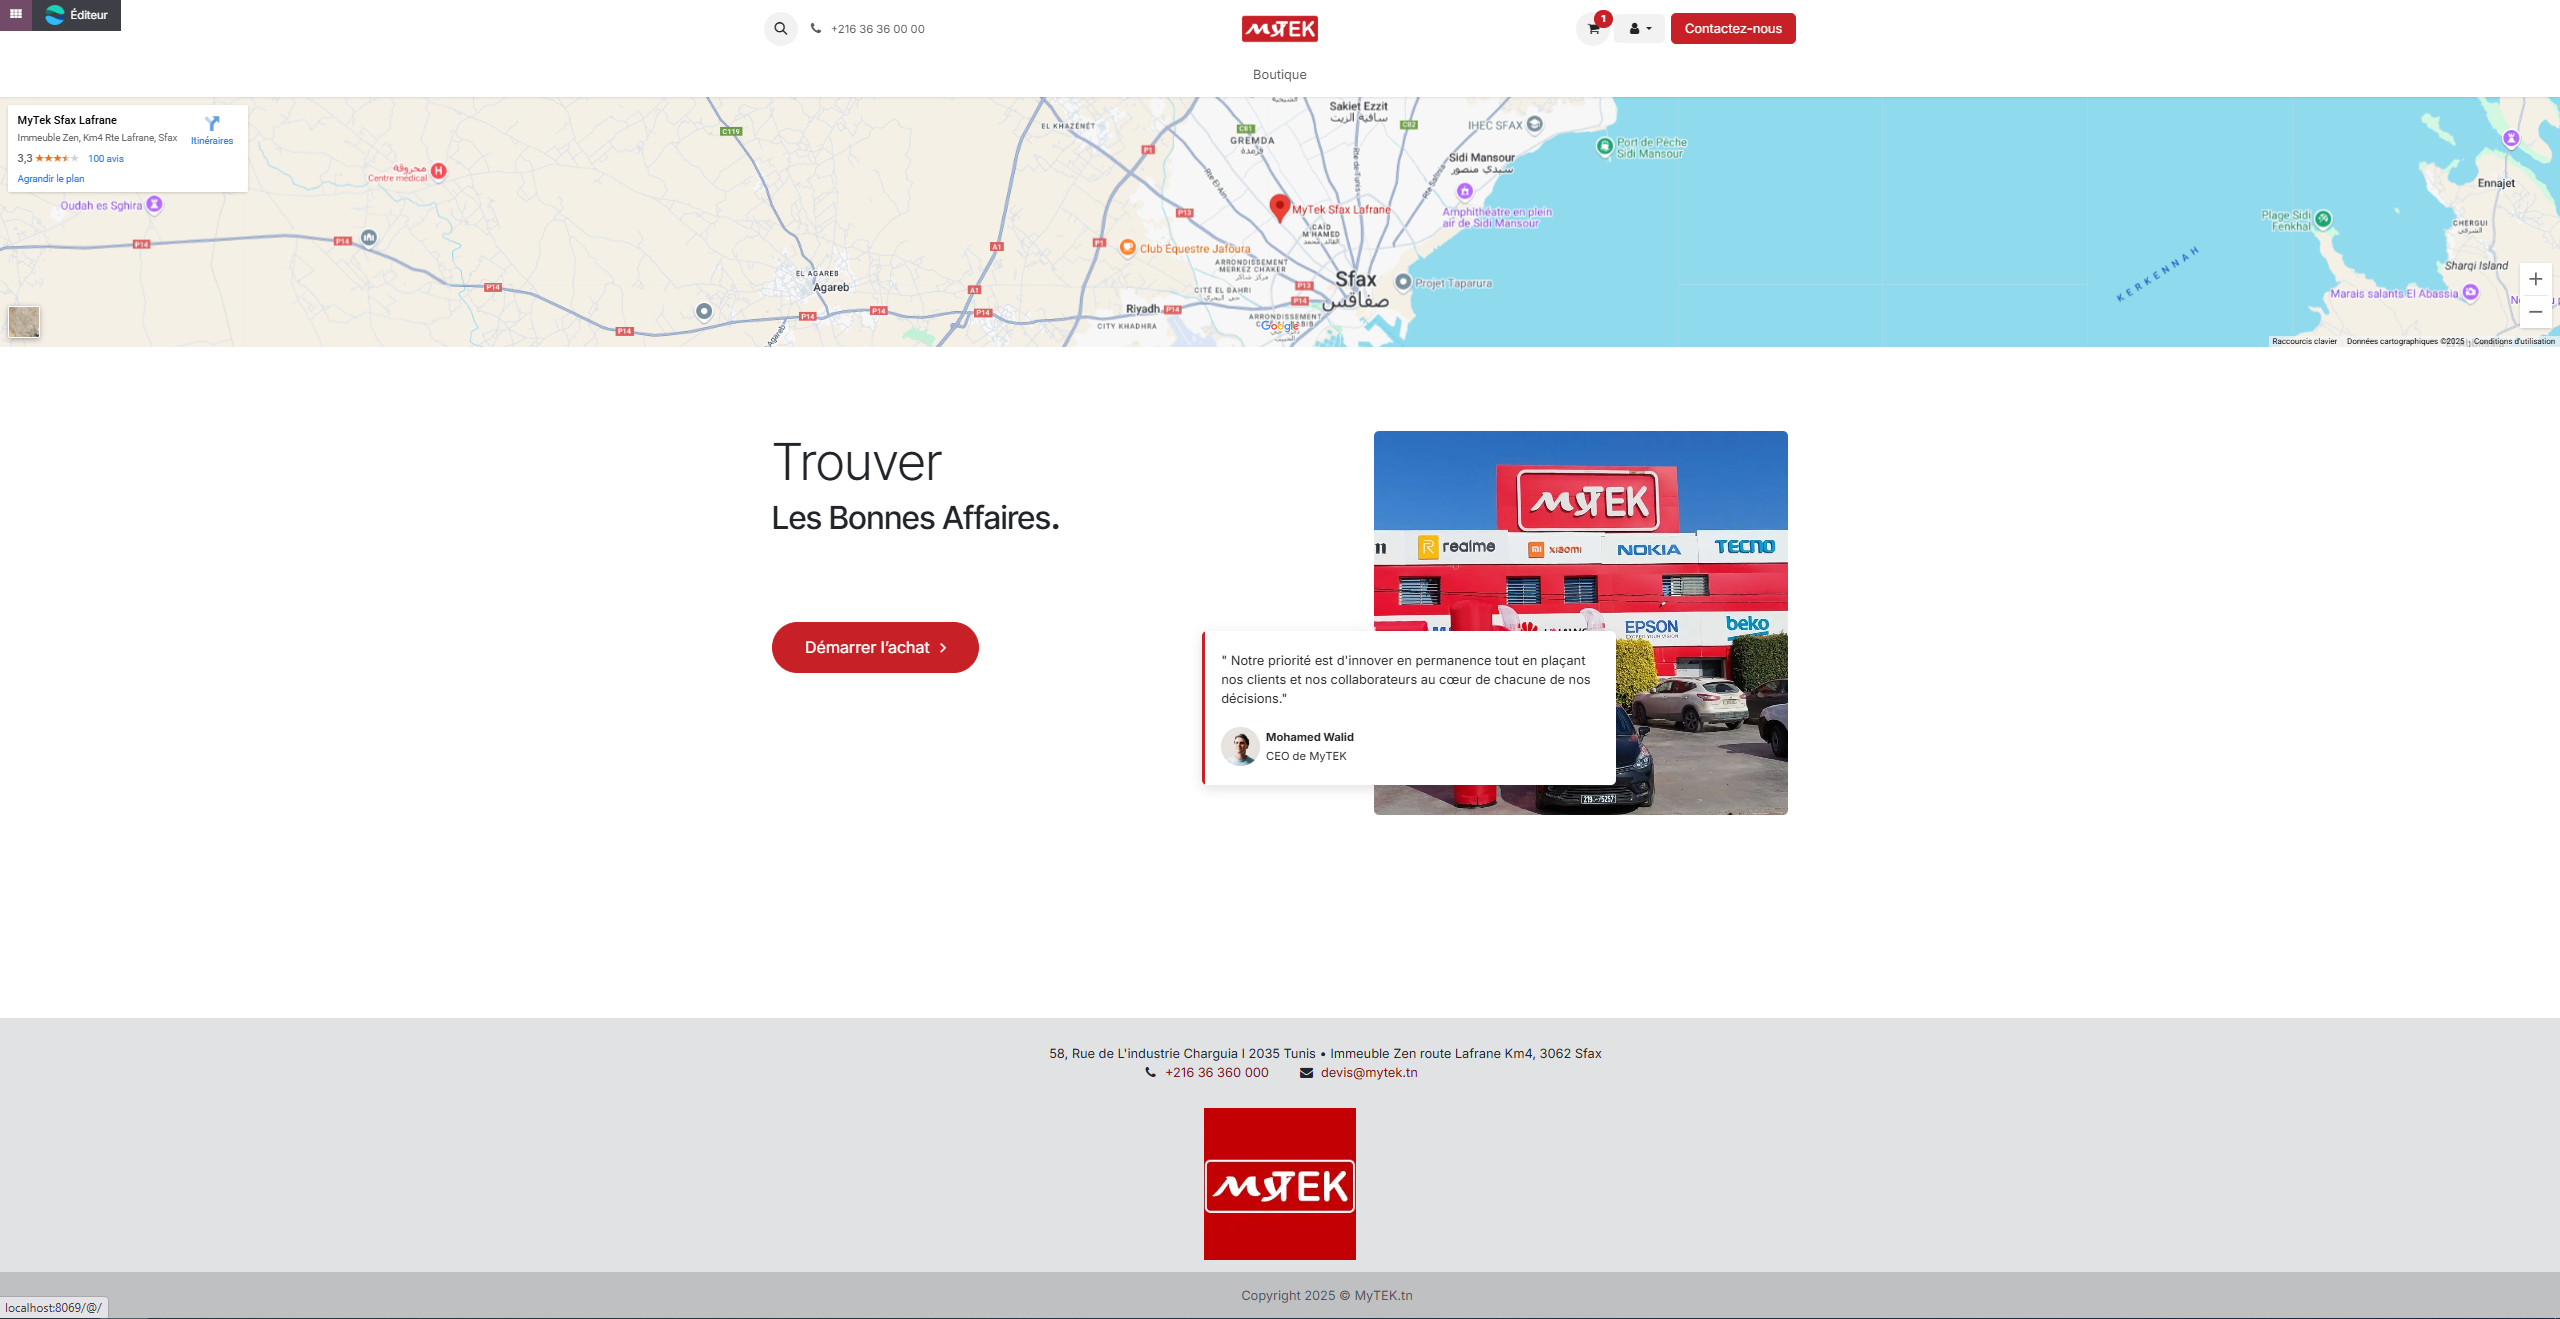
\includegraphics[width=0.8\textwidth]{images/interfaces/page_acceuil.PNG}
    \caption{Page d'accueil du site}
    \label{fig:page_accueil}
\end{figure}

La page d’accueil constitue la première impression du site. Elle offre un aperçu général de la société, met en avant la boutique la plus proche et présente les principales sections accessibles.

\begin{figure}[H]
    \centering
    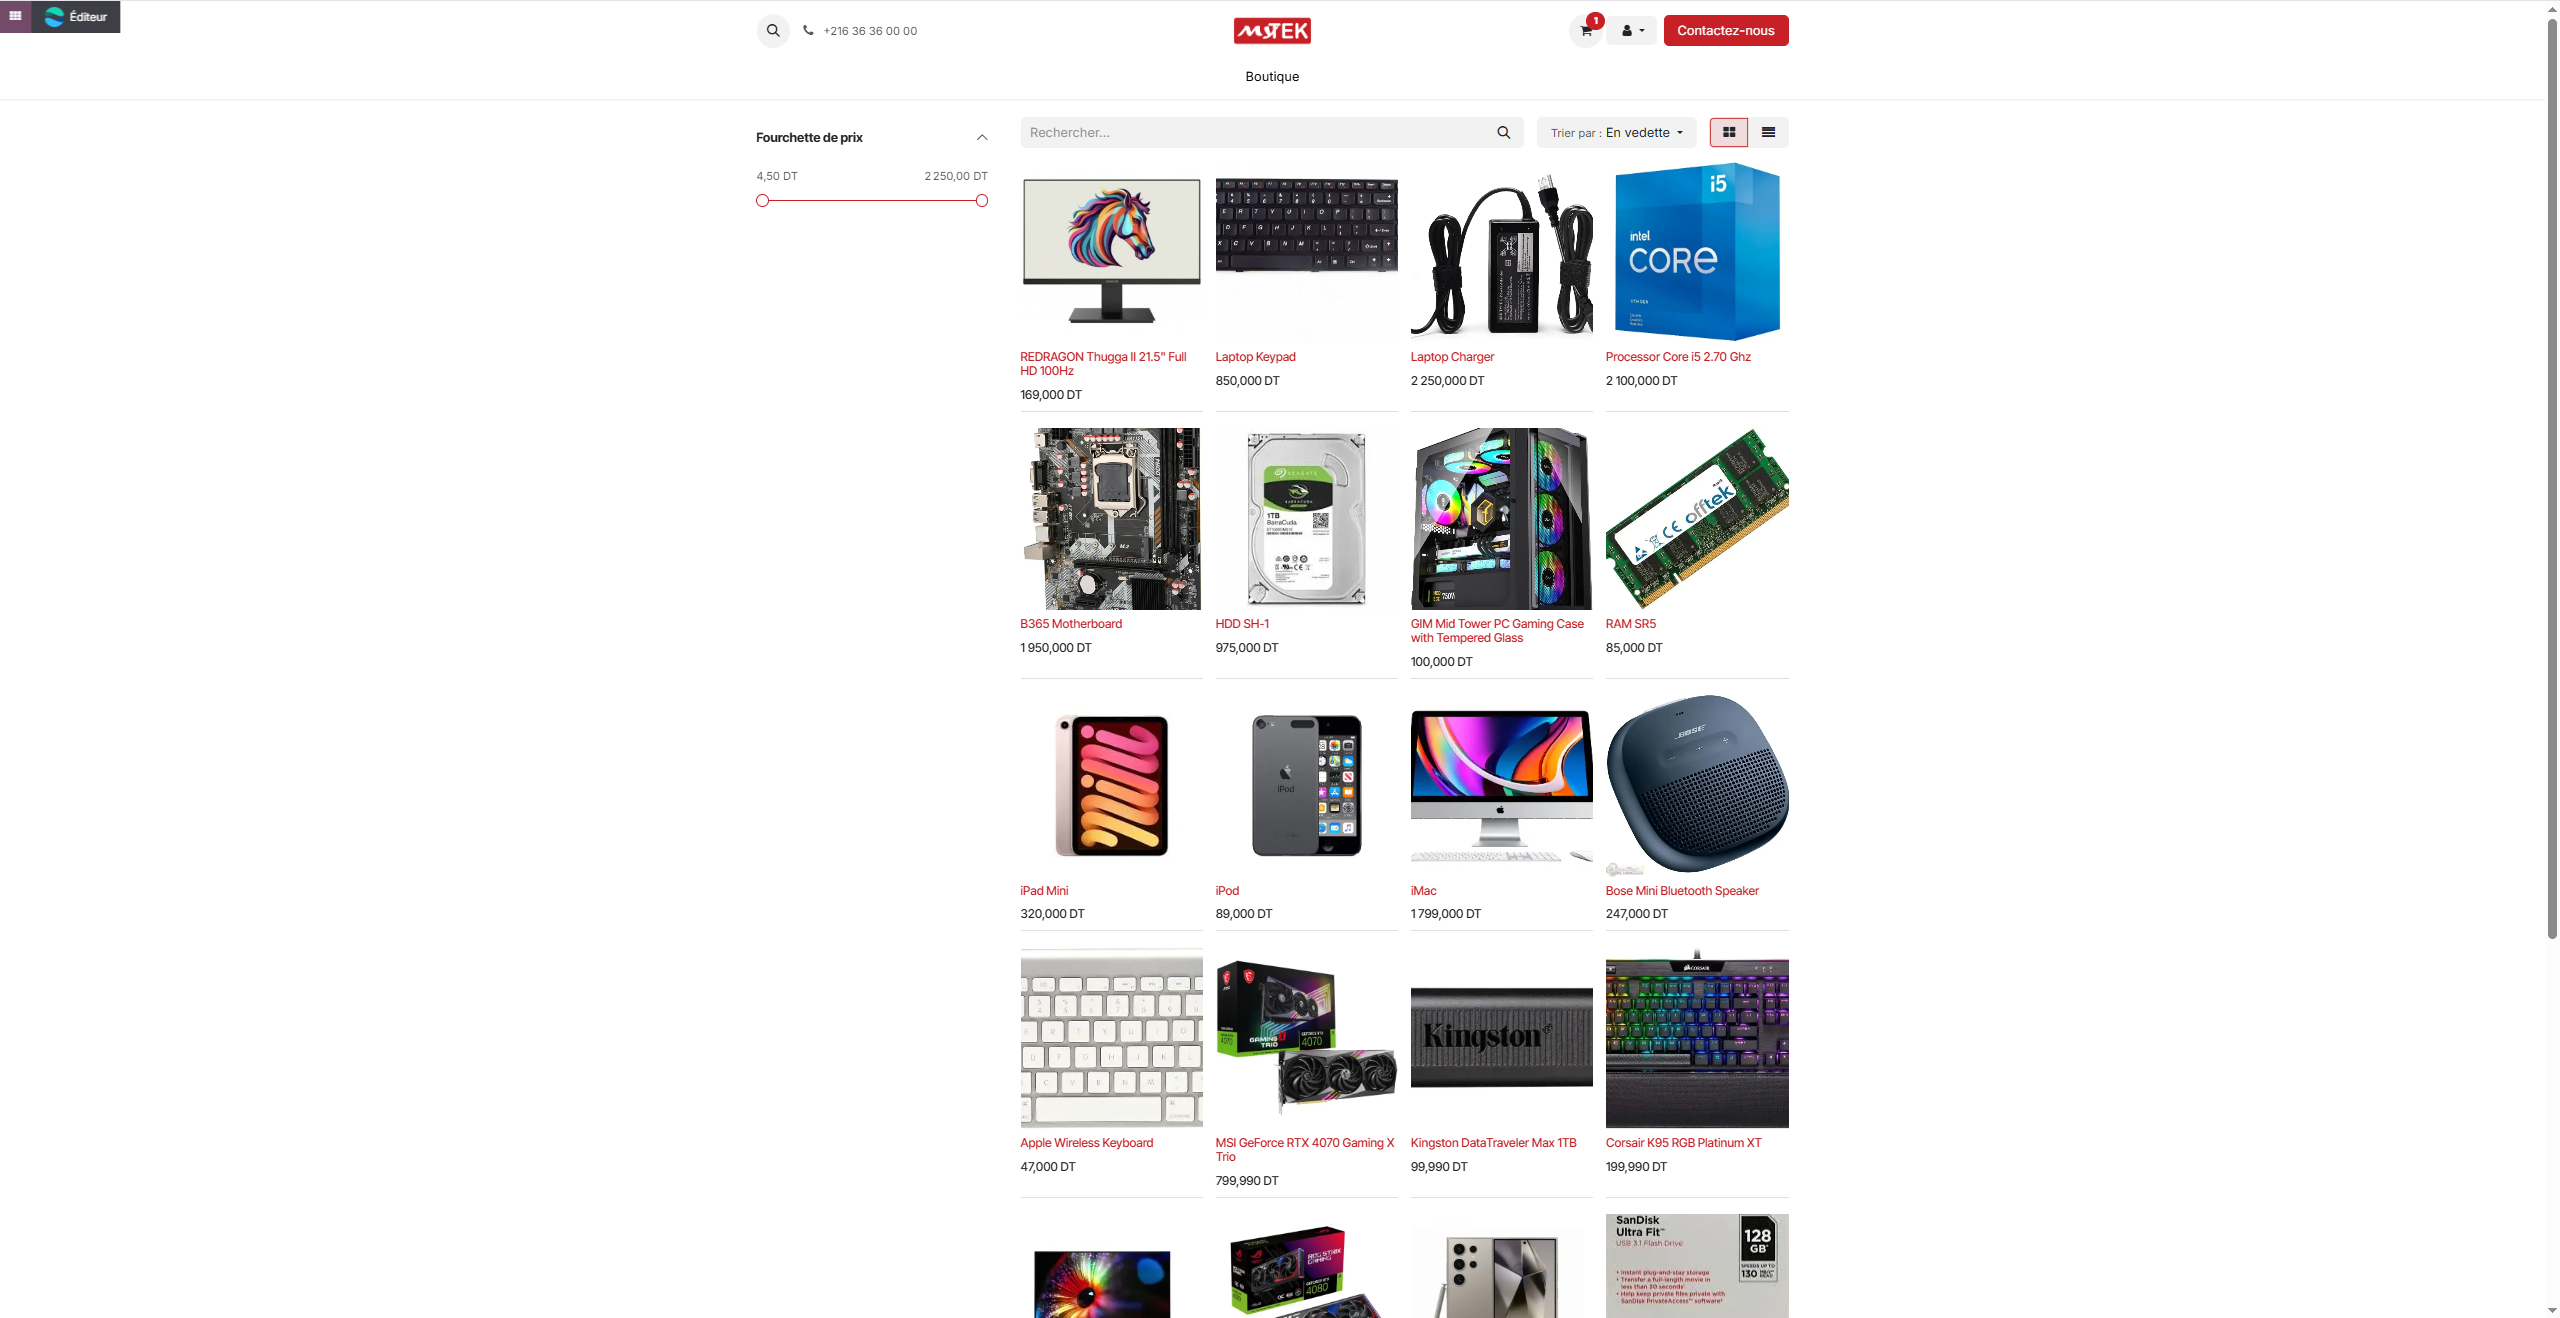
\includegraphics[width=0.8\textwidth]{images/interfaces/page_boutique.PNG}
    \caption{Page de la boutique en ligne}
    \label{fig:page_boutique}
\end{figure}

Cette page permet aux utilisateurs de parcourir les produits disponibles. Chaque article est présenté avec une image, son prix, ainsi qu’un lien vers sa fiche détaillée.

\begin{figure}[H]
    \centering
    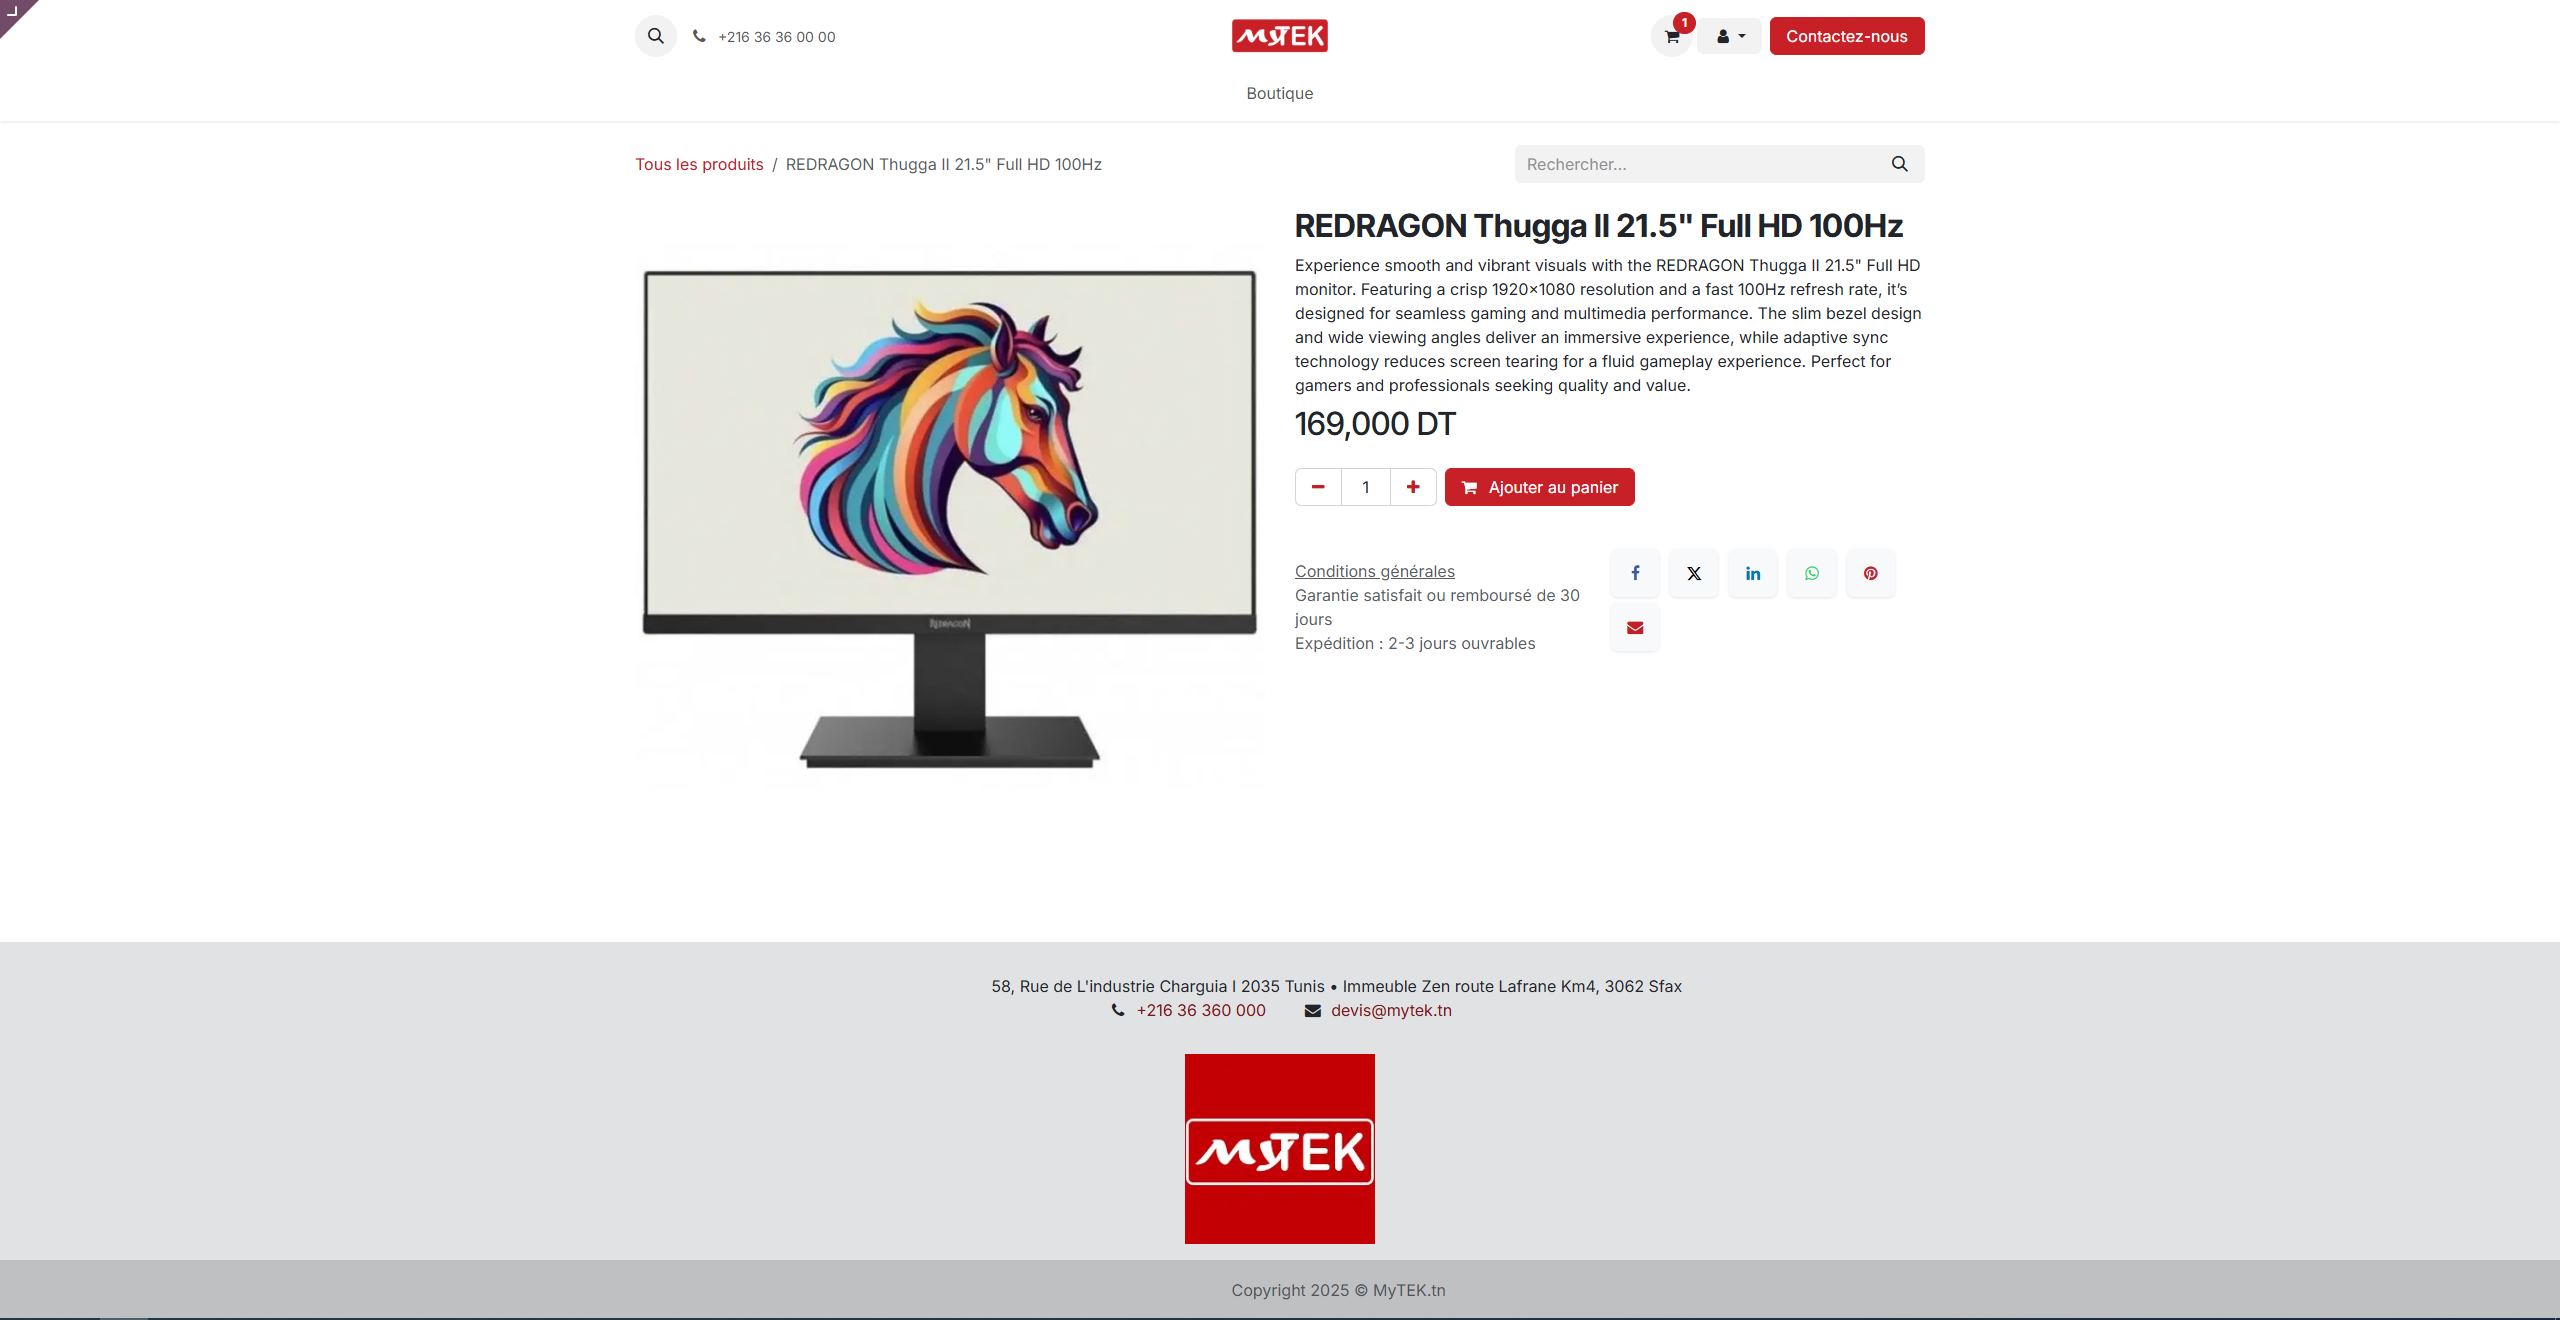
\includegraphics[width=0.8\textwidth]{images/interfaces/page_produit_details.PNG}
    \caption{Page de détails du produit}
    \label{fig:page_details_produit}
\end{figure}

La page de détails affiche les informations complètes d’un produit sélectionné, incluant sa description, ses caractéristiques techniques et, le cas échéant, les avis des clients.

\begin{figure}[H]
    \centering
    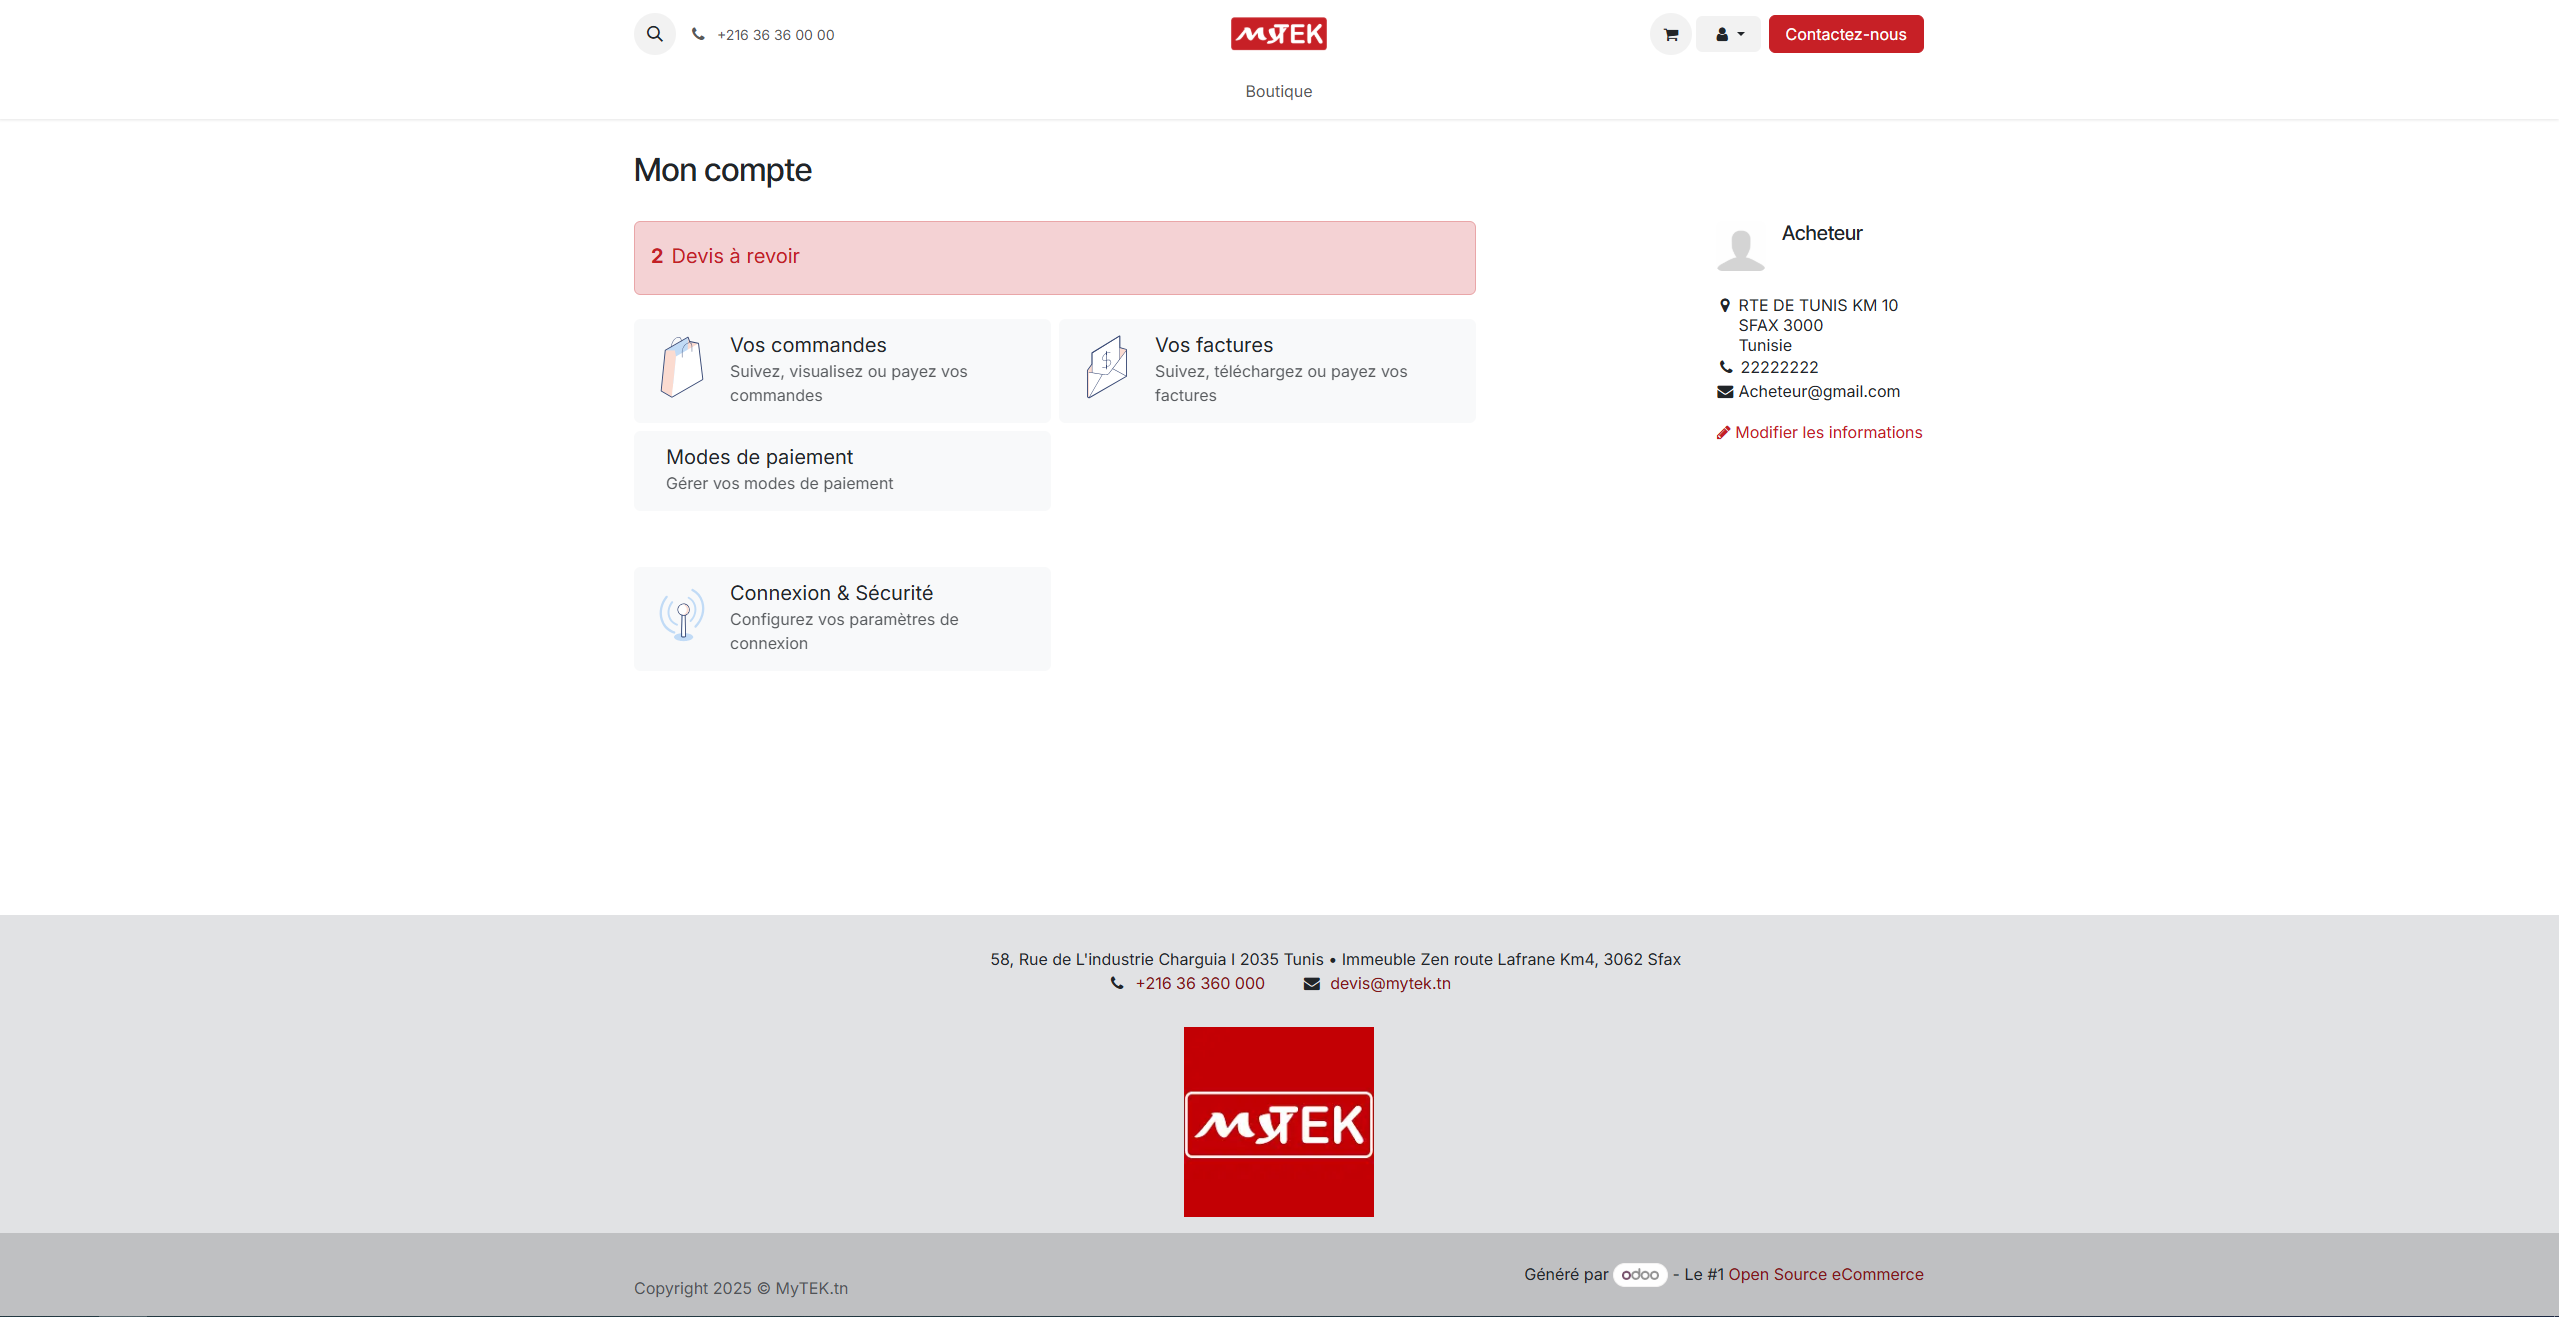
\includegraphics[width=0.8\textwidth]{images/interfaces/page_mon_compte.PNG}
    \caption{Page \og Mon compte \fg}
    \label{fig:page_mon_compte}
\end{figure}

La page \og Mon compte \fg{} permet à l’utilisateur de consulter et de modifier ses informations personnelles, de gérer ses commandes et de suivre l’historique de ses achats.

\begin{figure}[H]
    \centering
    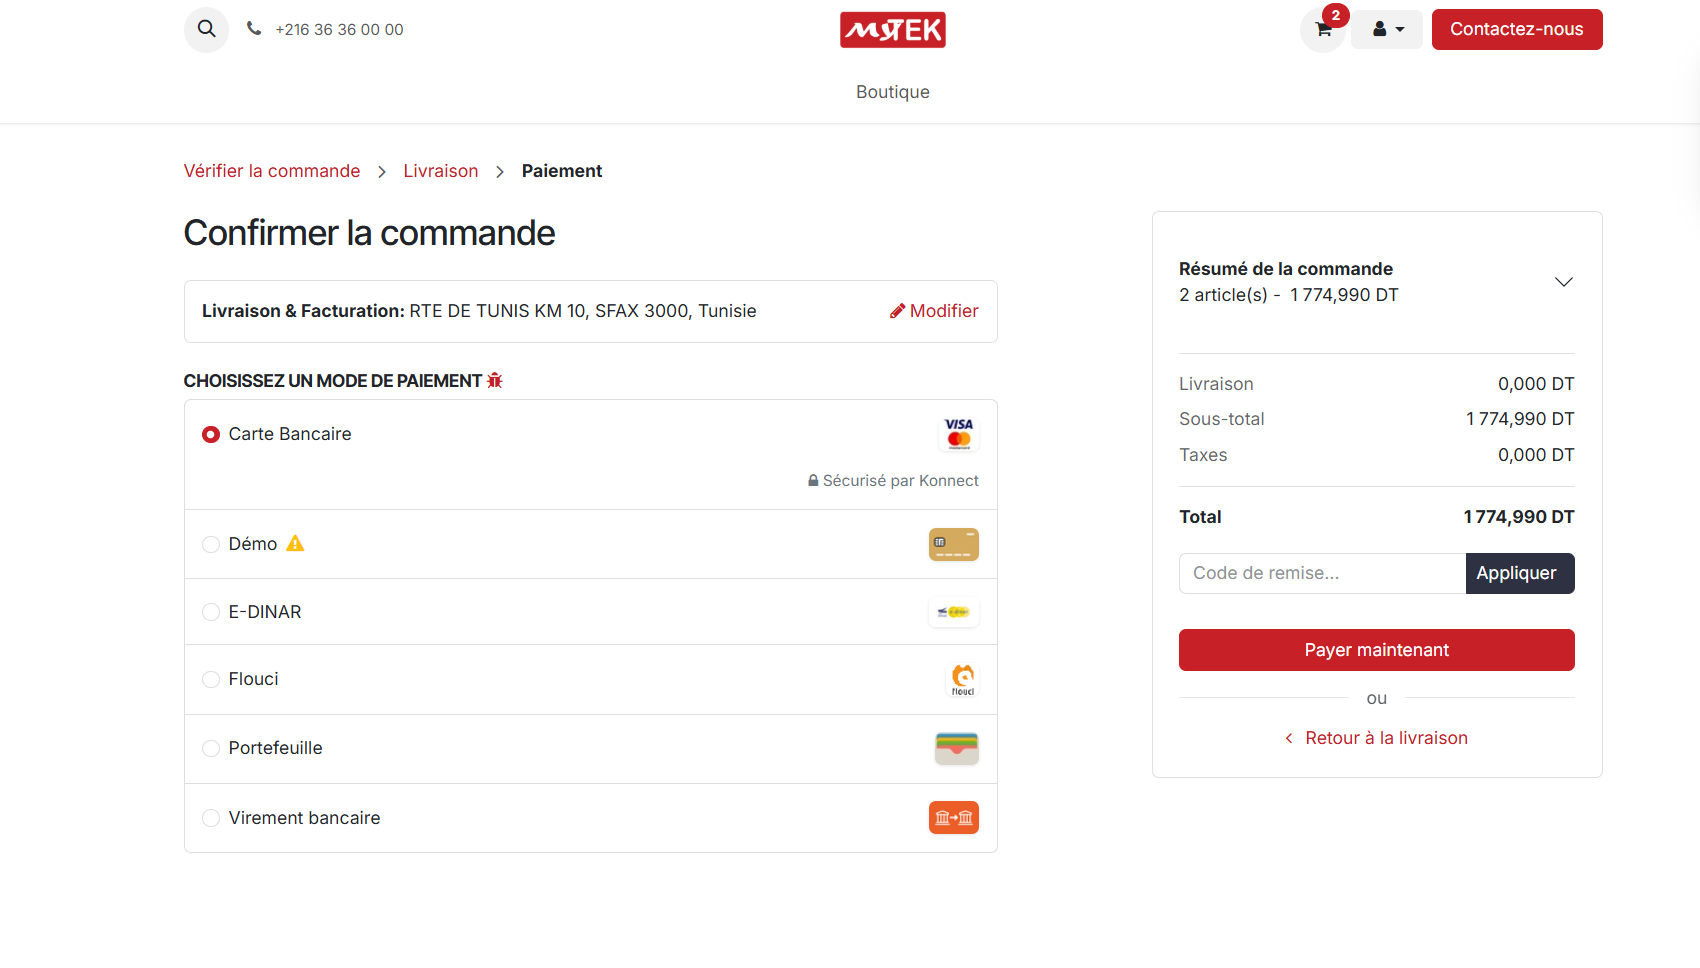
\includegraphics[width=0.8\textwidth]{images/interfaces/page_payer.PNG}
    \caption{Page de confirmation de commande}
    \label{fig:page_paiement}
\end{figure}

La page de paiement permet à l’utilisateur de finaliser sa commande en choisissant un mode de livraison et de paiement sécurisé. Elle constitue l’étape finale du processus d’achat, garantissant une expérience fluide et sécurisée.

\chapter{Conclusion et perspectives}

Ce projet a permis la mise en œuvre d’une solution intégrée de gestion commerciale à l’aide de l’ERP Odoo. Il s’est inscrit dans une démarche à la fois technique et fonctionnelle, avec pour objectif de couvrir l’ensemble du cycle de vente. Les réalisations majeures sont les suivantes :

\begin{itemize}
\item Déploiement d'une chaîne complète de gestion des ventes, incluant la création de produits, la gestion des devis, des commandes, de la facturation et des paiements ;
\item Exploration approfondie des possibilités de personnalisation offertes par les modules Odoo, tant sur le plan fonctionnel que sur le plan technique ;
\item Intégration de services externes tels que le protocole SMTP pour l’envoi automatisé de courriels et la mise en place de solutions de paiement en ligne, assurant une interopérabilité cohérente au sein de l’écosystème applicatif.
\end{itemize}

\bigskip

\textbf{Perspectives d’évolution :}

Afin d’augmenter le degré d’automatisation, d’efficacité et de performance de la solution, plusieurs axes d'amélioration ont été identifiés :

\begin{itemize}
\item Implémentation d’une gestion de stock dynamique, intégrant les seuils de réapprovisionnement et les alertes automatisées, afin d’optimiser la disponibilité des produits ;
\item Amélioration du référencement naturel (SEO) à travers l’optimisation du contenu, des balises méta et de la structure du site web, pour accroître la visibilité et le trafic organique ;
\item Connexion à un système logistique réel (via API ou ERP logistique tiers) dans le but de fluidifier le traitement des commandes, la gestion des expéditions et le suivi des livraisons.
\end{itemize}

\end{document}